\documentclass[11pt,a4paper]{article} % Prepara un documento con un font grande

\usepackage{iftex}

\ifLuaTeX
  % Adatta LaTeX alle convenzioni tipografiche italiane,
% e ridefinisce alcuni titoli in italiano, come "Capitolo" al posto di "Chapter",
% se il documento è in italiano
%\usepackage[italian]{babel}
%\usepackage[utf8]{inputenc} % Consente l'uso caratteri accentati italiani
%\usepackage{graphicx}		% Per le immagini
%\usepackage{gnuplot-lua-tikz}
%\usepackage[top=2.5cm, bottom=2cm, left=2cm, right=2cm]{geometry}

%\nonstopmode %non fermarti agli errori

%\usepackage{fancyhdr}
%\setlength{\headheight}{15.2pt}
%\pagestyle{fancy} % Solo le pagine normali, non i titoli nè la pagina iniziale


%%%%%%%%%%%%%%%%%%%%%%%%%%%%%%%%%%%%%%%%%%%%%%%%%%%%%%%%%%%%%%%%%%%%%%%%%%%%%%%%%%%%%%%%%

\usepackage{lipsum} % Package to generate dummy text throughout this template

\usepackage{fontspec}
\setmainfont[Ligatures=TeX]{Alegreya}

%\usepackage[sc]{mathpazo} % Use the Palatino font
%\usepackage[T1]{fontenc} % Use 8-bit encoding that has 256 glyphs
%%%%%
%\usepackage{Alegreya} %% Option 'black' gives heavier bold face 
%\renewcommand*\oldstylenums[1]{{\AlegreyaOsF #1}}

%\usepackage[euler-digits,euler-hat-accent]{eulervm}
%%%%%%
%\usepackage[utf8]{inputenc} % Consente l'uso caratteri accentati italiani
%\linespread{1.05} % Line spacing - Palatino needs more space between lines
\usepackage{amsmath, amsthm, amssymb, amsfonts}
\usepackage{microtype} % Slightly tweak font spacing for aesthetics

%%%%%%%%%%%%%%%%%%%%%%%%%%%%%%%%%%%%%%%%%%%%%
%Miei package
\usepackage[italian]{babel}
\usepackage{graphicx}		% Per le immagini
\usepackage{gnuplot-lua-tikz}
%%%%%%%%%%%%%%%%%%%%%%%%%%%%%%%%%%%%%%%%%%%%%
\usepackage[hmarginratio=1:1,top=32mm,columnsep=20pt]{geometry} % Document margins
\usepackage{multicol} % Used for the two-column layout of the document
\usepackage[hang, small,labelfont=bf,up,textfont=it,up]{caption} % Custom captions under/above floats in tables or figures
\usepackage{booktabs} % Horizontal rules in tables
\usepackage{float} % Required for tables and figures in the multi-column environment - they need to be placed in specific locations with the [H] (e.g. \begin{table}[H])
\usepackage{hyperref} % For hyperlinks in the PDF

\usepackage{lettrine} % The lettrine is the first enlarged letter at the beginning of the text
\usepackage{paralist} % Used for the compactitem environment which makes bullet points with less space between them

\usepackage{abstract} % Allows abstract customization
\renewcommand{\abstractnamefont}{\normalfont\bfseries} % Set the "Abstract" text to bold
\renewcommand{\abstracttextfont}{\normalfont\small\itshape} % Set the abstract itself to small italic text

\usepackage{titlesec} % Allows customization of titles
\renewcommand\thesection{\Roman{section}} % Roman numerals for the sections
\renewcommand\thesubsection{\Roman{subsection}} % Roman numerals for subsections
\titleformat{\section}[block]{\large\scshape\centering}{\thesection.}{1em}{} % Change the look of the section titles
\titleformat{\subsection}[block]{\large}{\thesubsection.}{1em}{} % Change the look of the section titles

\usepackage{fancyhdr} % Headers and footers
\pagestyle{fancy} % All pages have headers and footers
\fancyhead{} % Blank out the default header
\fancyfoot{} % Blank out the default footer
\fancyhead[C]{Running title $\bullet$ November 2012 $\bullet$ Vol. XXI, No. 1} % Custom header text
\fancyfoot[RO,LE]{\thepage} % Custom footer text


\else
  % Adatta LaTeX alle convenzioni tipografiche italiane,
% e ridefinisce alcuni titoli in italiano, come "Capitolo" al posto di "Chapter",
% se il documento è in italiano
%\usepackage[italian]{babel}
%\usepackage[utf8]{inputenc} % Consente l'uso caratteri accentati italiani
%\usepackage{graphicx}		% Per le immagini
%\usepackage{gnuplot-lua-tikz}
%\usepackage[top=2.5cm, bottom=2cm, left=2cm, right=2cm]{geometry}

%\nonstopmode %non fermarti agli errori

%\usepackage{fancyhdr}
%\setlength{\headheight}{15.2pt}
%\pagestyle{fancy} % Solo le pagine normali, non i titoli nè la pagina iniziale


%%%%%%%%%%%%%%%%%%%%%%%%%%%%%%%%%%%%%%%%%%%%%%%%%%%%%%%%%%%%%%%%%%%%%%%%%%%%%%%%%%%%%%%%%

\usepackage{lipsum} % Package to generate dummy text throughout this template

\usepackage[sc]{mathpazo} % Use the Palatino font
%\usepackage{tgpagella} % TeX Gyre Pagella, versione migliorata di Palatino. Si ma bo, no
%\usepackage{inconsolata}
\usepackage{textcomp}
\usepackage[scale=0.98,ttdefault]{AnonymousPro}

%%%%%
%\usepackage{Alegreya} %% Option 'black' gives heavier bold face 
\usepackage{AlegreyaSans} %% Option 'black' gives heavier bold face 
%\renewcommand*\oldstylenums[1]{{\AlegreyaOsF #1}}
\usepackage{opensans}
%\usepackage[euler-digits,euler-hat-accent]{eulervm}
\usepackage[euler-hat-accent]{eulervm}
%%%%%%

\usepackage[T1]{fontenc} % Use 8-bit encoding that has 256 glyphs

\usepackage[utf8]{inputenc} % Consente l'uso caratteri accentati italiani
\linespread{1.08} % Line spacing - Palatino needs more space between lines, messo a 1.05 da 1.11 che era per alegreya
\usepackage{amsmath, amsthm, amssymb, amsfonts}
\usepackage[italian]{babel}
%\usepackage[kerning,spacing,tracking,letterspace = 2,babel]{microtype} % Slightly tweak font spacing for aesthetics. Il tre è pensato per Alegreya
\usepackage[kerning,spacing,babel]{microtype}
%\SetTracking[]{encoding = *,shape = *}{3} % Aumenta la distanza fra le lettere
							     % http://tex.stackexchange.com/questions/66494/new-command-for-spacing-letters-in-microtype
%%%%%%%%%%%%%%%%%%%%%%%%%%%%%%%%%%%%%%%%%%%%%
%Miei package



\usepackage{graphicx}		% Per le immagini
\usepackage{fixltx2e}
%\usepackage{color}		% COLORI!

%\definecolor{grigio-molto-scuro}{gray}{0.1}	%colore

\usepackage{tabularx}		% Per le tabelle con le colonne tutte uguali
\usepackage{tabulary}		% Tabelle migliorate, nelle celle il testo va a capo da solo...
\usepackage{gnuplot-lua-tikz}
%%%%%%%%%%%%%%%%%%%%%%%%%%%%%%%%%%%%%%%%%%%%%
\newlength{\alphabet}
\settowidth{\alphabet}{\normalfont abcdefghijklmnopqrstuvwxyz}
\usepackage[
	    %hmargin=0.18\paperwidth,% metti la larghezza del testo (margini orizzontali) al 18% del foglio
	    textwidth=2.4\alphabet,  % http://tex.stackexchange.com/questions/59626/nicely-force-66-characters-per-line
	    hmarginratio=1:1,       % margini destro e sinistro uguali
	    top=35mm,	            % margine sopra a 32mm...
	    vmarginratio=4:5,       % quello sotto uguale (default 2:3)
	    columnsep=20pt]         % Spazio tra le colonne?
	    {geometry} % Document margins
\usepackage{multicol} % Used for the two-column layout of the document
\usepackage[hang, small,labelfont=bf,up,textfont=it,up]{caption} % Custom captions under/above floats in tables or figures
\usepackage{booktabs} % Horizontal rules in tables
\usepackage{float} % Required for tables and figures in the multi-column environment - they need to be placed in specific locations with the [H] (e.g. \begin{table}[H])
\usepackage[hidelinks]{hyperref} % For hyperlinks in the PDF
\usepackage{nicefrac} % Per le frazioni tipo ⅛
\usepackage{pdfpages} % Per includere pagine intere in pdf (per la copertina)
%\usepackage[squaren]{siunitx}

\usepackage{lettrine} % The lettrine is the first enlarged letter at the beginning of the text
\usepackage{paralist} % Used for the compactitem environment which makes bullet points with less space between them
\usepackage[section]{placeins} % Per \FloatBarrier. L'opzione section comporta che le sezioni siano floatbarriers

\usepackage{abstract} % Allows abstract customization
\renewcommand{\abstractnamefont}{\normalfont\bfseries} % Set the "Abstract" text to bold
\renewcommand{\abstracttextfont}{\normalfont\small\itshape} % Set the abstract itself to small italic text

\usepackage{caption} % Per captions avanzate

\usepackage{listingsutf8} % Per includere codice sorgente meglio che con verbatim (e con caratteri non inglesi)
\lstset{ 
  %Preso anche questo da http://en.wikibooks.org/wiki/LaTeX/Source_Code_Listings
  %backgroundcolor=\color{white},   % choose the background color; you must add \usepackage{color} or \usepackage{xcolor}
  basicstyle=\footnotesize\ttfamily,        % the size of the fonts that are used for the code E MESSO IN MONOSPACE
  breakatwhitespace=true,         % sets if automatic breaks should only happen at whitespace
  breaklines=true,                 % sets automatic line breaking
  captionpos=b,                    % sets the caption-position to bottom
  %commentstyle=\color{mygreen},    % comment style
  %deletekeywords={...},            % if you want to delete keywords from the given language
  %escapeinside={\%*}{*)},          % if you want to add LaTeX within your code
  %extendedchars=true,              % lets you use non-ASCII characters; for 8-bits encodings only, does not work with UTF-8
  frame=l,                    % adds a frame around the code
				    %you can control the rules at the top, right, bottom, and left directly by using the four initial 
				    %letters for single rules and their upper case versions for double rules. http://mirror.hmc.edu/ctan/macros/latex/contrib/listings/listings.pdf
				    % Es frame frame=trBL ha doppia linea a sinistra e sotto, e singola a destra e sopra
  keepspaces=true,                 % keeps spaces in text, useful for keeping indentation of code (possibly needs columns=flexible)
  %keywordstyle=\color{blue},       % keyword style
  %language=Octave,                 % the language of the code
  %morekeywords={*,...},            % if you want to add more keywords to the set
  numbers=left,                    % where to put the line-numbers; possible values are (none, left, right)
  numbersep=5pt,                   % how far the line-numbers are from the code
  %numberstyle=\tiny\color{mygray}, % the style that is used for the line-numbers
  %rulecolor=\color{black},         % if not set, the frame-color may be changed on line-breaks within not-black text (e.g. comments (green here))
  showspaces=false,                % show spaces everywhere adding particular underscores; it overrides 'showstringspaces'
  showstringspaces=false,          % underline spaces within strings only
  showtabs=false,                  % show tabs within strings adding particular underscores
  stepnumber=2,                    % the step between two line-numbers. If it's 1, each line will be numbered
  %stringstyle=\color{mymauve},     % string literal style
  tabsize=2,                       % sets default tabsize to 2 spaces
  title=\lstname                   % show the filename of files included with \lstinputlisting; also try caption instead of title
}


\usepackage{titlesec} % Allows customization of titles
\renewcommand\thesection{\Roman{section}} % Roman numerals for the sections
\renewcommand\thesubsection{\Roman{subsection}} % Roman numerals for subsections
% \usefont {encoding} {family} {series} {shape}
\titleformat{\section}[block]{\AlegreyaSansSC \bfseries \LARGE}{\thesection.}{1em}{} % Change the look of the section titles. Pezzi spostati \scshape\centering\bfseries
\titleformat{\subsection}[block]{\AlegreyaSans \bfseries \Large}{\thesection.\thesubsection }{1em}{} % Change the look of the section titles

\usepackage{fancyhdr} % Headers and footers
\pagestyle{fancy} % All pages have headers and footers
\fancyhead{} % Blank out the default header
\fancyfoot{} % Blank out the default footer
\headheight=14pt % Perchè sennò continua a lamentarsi che 12pt è troppo poco e la mette a 14 lo stesso
\fancyhead[C]{Chiappara, Labanca, Forcher - \textit{Ottica geometrica} $\bullet$ \thesection} % Custom header text. \nouppercase{\leftmark} per sezione, ma non ci sta
\fancyfoot[RO,LE]{\thepage} % Custom footer text


\fi
\DeclareGraphicsExtensions{.pdf, .png, .jpg} % Se due immagini hanno lo stesso nome sceglile secondo l'ordine di filetype qui
\graphicspath{ {./img/} }					 % Path delle immagini 

\input{./preamboli_e_stili/titolo_Pendolo_Torsione.tex}
%%%%%%%%%%%%%%%%%%%%%%%%%%%%%%%%%%%%%%5%%%%%%%%%%%%%%%%%%%%%%%%%%%%%%%%%%%%%%%%%%%
\usepackage{float}
\usepackage{caption}
%\usepackage{multirow}
%\usepackage[top=3.6cm, bottom=1.5in, left=0.5in, right=0.5in]{geometry}

% I miei stili di float, con le righe
\floatstyle{plaintop}
\newfloat{tabella}{tb}{lop}
\floatname{tabella}{Tabella}

\floatstyle{ruled}
\newfloat{grafico}{tb}{log}
\floatname{grafico}{Grafico}

\newcommand{\tabellaautorefname}{\bfseries Tabella} % per \autoref del package hyperref
\newcommand{\graficoautorefname}{\bfseries Grafico} % Idem
%%%%%%%%%%%%%%%%%%%%%%%%%%%%%%%%%%%%%%%%%%%%%%%%%%%%%%%%%%%%%%%%%%%%%5%%%%%%%%%%%%%

\newcommand{\cm}{\,\mathrm{cm}}
\DeclareMathOperator{\cov}{cov} % Covarianza
\DeclareMathOperator{\var}{var} % Covarianza
\newcommand{\mm}{\,\mathrm{mm}}
\newcommand{\nm}{\,\mathrm{nm}}
\newcommand{\usuq}{\nicefrac{1}{q}}
\newcommand{\usup}{\nicefrac{1}{p}}



%////////////////////////////////////////////////////////////////////////////////////////////////////////////////////////////
%////////////////////////////////////////////////////////////////////////////////////////////////////////////////////////////
% Fine dei dati iniziali per il latex: il documento finale inizierà da qui
\begin{document}

{
\color{grigio-molto-scuro}
%\lsstyle % Abilita il letterspacing personalizzato
%\unclfamily % Cagata per il font Uncial

\maketitle % Produce il titolo a partire dai comandi \title, \author e \date

\vspace{ \stretch{1} }
\begin{center}
	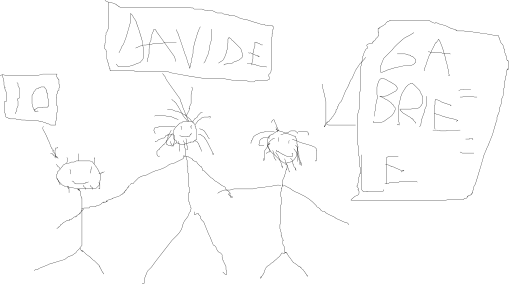
\includegraphics[width=0.7\textwidth]{gruppo_rel}
\end{center}

\vspace{ \stretch{1} }
% Le varie sezioni
%\section{Obiettivi}
\begin{abstract}
	\noindent
	L'obiettivo delle esperienze \`e la stima delle grandezze fisiche 
caratterizzanti la lente presa in considerazione, la numero 3. Con 
le prime tre esperienze si sono trovate altrettante stime della 
distanza focale $f^{\star}$, le quali sono state utilizzate, una volta 
corrette rispetto all'aberrazione sferica, per la stima del 
coefficiente $c$ di tale aberrazione (quarta esperienza) e del 
numero di Abbe $V$, indicativo all'aberrazione cromatica (quinta 
esperienza).

\end{abstract}

\newpage


\microtypesetup{protrusion=false} % disables protrusion locally in the document
\tableofcontents % prints Table of Contents
\microtypesetup{protrusion=true} % enables protrusion

%\begin{multicols}{2}

\section{Apparato strumentale}
	La strumentazione (banco ottico numero 5) consisteva in:
\begin{compactitem}
\item Guida ottica di lunghezza $\approx 140 \cm$ con scala graduata con passo 0.5 mm
\item Generatore di corrente di intensità e voltaggio regolabili
\item Lampada 
\item Cavaliere portalampada con tre filtri cromatici e un portamascherine
\item Cavaliere portalente con micrometro (valore di azzeramento $8.60 \mm$)
\item Cavaliere portalente senza micrometro
\item Cavaliere portaschermo con due micrometri
\item Cavaliere portasquadra
\item Mascherina con buco centrale
\item Diaframma con singolo buco centrale
\item Diaframma con 2 buchi marginali e 2 parassiali posti su segmenti ortogonali
\item Lente numero 3
\item Doppietto di Dollond
\item Oculare con un ingrandimento di 8x
\end{compactitem}


\section{Metodologia di misura}
	L'esperienza \`e suddivisa in 5 fasi diverse, ognuna con 
un approccio sperimentale e un'analisi dati differenti. Questa 
sezione ha lo scopo di descrivere la metodologia prescelta dagli 
sperimentatori in laboratorio, dunque non vi si discutono le scelte 
numeriche fatte o le analisi dati, un'accurata descrizione delle 
quali è fornita nelle sezioni successive.

Preliminarmente a ogni esperienza, è stato necessario preparare il 
banco ottico con la seguente procedura: in primo luogo tutti i 
micrometri sono stati portati allo zero della scala, dopodichè il 
cavaliere portalampada \`e stato fissato in un punto arbitrario della 
guida; tale punto è stato scelto il più marginalmente possibile 
sulla sinistra per avere spazio a disposizione per gli altri 
cavalieri. Bloccato con la vite il cavaliere portalampada, si 
\`e utilizzato il cavaliere con squadra per andare a leggere sulla scala 
millimetrata il valore che, dopo aver finito la preparazione 
dell'apparato sperimentale, indica la posizione 
dell'oggetto relativa alla guida ottica. Il cavaliere con squadra \`e stato subito
 rimosso dalla guida ottica. Fatto ciò, si \`e montata la 
mascherina con foro singolo sull'apposito supporto presente sul 
cavaliere portalampada, mantenendo l'anello di fissaggio rivolto a 
destra.

Sistemato il cavaliere portalampada, il cavaliere 
portalente \`e stato posizionato sulla guida ottica e vi si sono avvitati la 
lente sul lato destro, poi il diaframma sul sinistro. \`E stata posta 
particolare attenzione nell'avvitare la lente fino alla fine del 
filo delle componenti meccaniche del sistema. Alla destra del 
portalente non ancora fissato \`e stato posto il cavaliere portaschermo con 
micrometro, in modo tale che lo schermo fosse rivolto verso sinistra, 
e si \`e inserito nel cavaliere portalampada il filtro di colore giallo.

\subsection{Autocollimazione}
Per stimare la lunghezza focale attraverso il metodo 
dell'autocollimazione si è operato spostando il cavaliere portalente 
con micrometro sulla guida ottica manualmente o attraverso il 
micrometro, leggendo i valori dal metro posto sulla guida 
o sui micrometri. Il diaframma utilizzato per questa esperienza è 
quello con un singolo foro centrale. 

Preparato il banco 
ottico, prima di iniziare la vera e propria presa dati si è cercato 
approssimativamente quale potesse essere la posizione del fuoco 
della lente. Si è quindi mosso il cavaliere portalente e 
successivamente confrontata grossolanamente la dimensione delle 
proiezioni del raggio sullo schermo, quando esso veniva posto vicino 
o lontano dal cavaliere portalente. Questa 
operazione è stata ripetuta più volte muovendo il cavaliere 
portalente a sinistra o a destra a seconda che l'immagine nello 
schermo fosse più grande rispettivamente nel caso lo schermo fosse 
posto più vicino o più lontano dalla lente. Una reiterazione di 
queste azioni ha permesso dopo circa 4-5 ripetizioni di trovare un 
punto per il cavaliere portalente per il quale il cerchio proiettato 
sullo schermo fosse di grandezza approssimativamente costante al 
muoversi del cavaliere portaschermo. 

Trovato il punto, ci si è spostati a destra di circa mezzo centimetro (iniziando con il 
valore zero della scala del micrometro sono possibili infatti solo 
spostamenti dello stesso che avvicinino la lente alla lampada e non 
c'è modo di allontanarle) e si è saldamente bloccato il cavaliere 
portalente con l'apposita vite. Il valore letto dall'indice del 
cavaliere portalente è stato registrato e poi è stata iniziata la 
presa dati. Per prima cosa è stato regolato il 
micrometro in modo tale che la lente fosse spostata di circa mezzo 
centimetro, in modo cioè che si trovasse sul punto nel quale a 
occhio era stata individuata la condizione di fascio parallelo. 
Successivamente, si è misurato il diametro a posizioni costanti 
dello schermo (da vicino, $30\cm$; da lontano, $130\cm$). Per fare 
ciò, è stato utilizzato il reticolo presente sullo schermo 
smerigliato: operando con il micrometro che permette allo schermo 
uno spostamento perpendicolare all'asse ottico, sono state misurate 
le posizioni che esso segnava quando una linea del reticolo 
diventava tangente al cerchio luminoso. Presi i dati, il diametro 
del cerchio \`e stato ottenuto sommando un centimetro alla 
differenza, procedura dedotta evidentemente	 dalla costruzione fisica 
del sistema. Confrontando i dati con la stessa logica dei passaggi 
precedenti, anche grazie a un programma che consentiva di 
visualizzarli istantaneamente su un grafico, si è spostata la lente 
avvicinandola o allontanandola dall'oggetto andando a operare sul 
micrometro presente nel cavaliere portalente. Trovato il punto in 
cui la differenza tra il diametro proiettato sullo schermo più 
distante e quello proiettato sullo schermo più prossimo cambiasse 
segno, si è indagato con maggiore precisione sull'area compresa tra 
le due misurazioni.

\subsection{Punti coniugati} 
Per trovare il fuoco attraverso il metodo dei punti coniugati, il 
cavaliere portalampada \`e stato bloccato, ma, a differenza dell'esperienza 
precedente, non si è bloccato il cavaliere portalente. Si è 
operato senza micrometri, solamente spostando i cavalieri lungo la 
guida ottica, e come nell'esperienza precedente si è utilizzato il 
diaframma con singolo buco centrale. Preparato il banco ottico si è 
posto il cavaliere portalente inizialmente a una distanza dal 
cavaliere portalampada maggiore del fuoco che era stato stimato con 
il metodo dell'autocollimazione. Muovendo il cavaliere portaschermo 
si è cercato il punto in cui il raggio proiettato presentasse 
diametro più piccolo possibile (per vederlo con più facilità si è 
fatto uso dell'oculare in dotazione), a quel punto si sono 
registrati su una tabella la posizione del cavaliere portalente e 
quella del cavaliere portaschermo. Il cavaliere portalente è stato 
poi allontanato dall'oggetto e si è ripetuta l'operazione, aggiungendo una 
riga alla tabella precedentemente fatta. Il processo è stato 
ripetuto indagando il più uniformemente possibile le posizioni 
permesse dalla guida ottica.

\subsection{Bessel}
Per trovare il fuoco attraverso il metodo di Bessel, sono stati 
tenuti fermi i cavalieri portalampada e portaschermo e si è 
mosso solamente il cavaliere portalente. Si è preparato il banco 
ottico e utilizzato il diaframma con buco singolo e il cavaliere 
portalente senza micrometro. Per prima cosa, data l'analisi teorica 
che si può fare a riguardo, si è bloccato il cavaliere portalampada 
il più a sinistra possibile e, 
utilizzando le stime fatte con le altre esperienze, si è bloccato il 
cavaliere portaschermo a più di 4f. Muovendo il cavaliere 
portalente, si sono cercate le due posizioni per cui l'immagine 
andasse a fuoco. Nel caso non risultasse evidente distinguere un 
fuoco dall'altro si è allontanato ulteriormente il cavaliere 
portaschermo. Trovata una posizione dei due cavalieri fissi tale che 
i due fuochi fossero facilmente distinguibili e i cavalieri non 
fossero troppo lontani tra loro, si è iniziata la presa dati. 
Aiutandosi con l'oculare, è stata misurata la posizione della lente 
per la quale il fascio andasse a fuoco sullo schermo. Spostando il 
cavaliere portalente è stato successivamente registrato il punto 
in cui l'immagine andasse nuovamente a fuoco nonostante la posizione 
fosse diversa. Tali misurazioni di posizione sono stati ripetute 10 
volte ciascuna.

\subsection{Aberrazione sferica}
Dopo le varie stime del fuoco, si sono cercate l'aberrazione sferica 
e l'aberrazione cromatica della lente. Per quanto riguarda 
l'aberrazione sferica, si è preparato il banco ottico utilizzando, 
differentemente rispetto ai casi precedenti, entrambi 
i cavalieri portalente: quello con micrometro portante il doppietto 
di Dollond e quello senza micrometro portante la lente. Inizialmente 
non è stato montato alcun diaframma ed è stato posizionato sulla 
guida ottica solamente il cavaliere con il doppietto acromatico. 
Grazie ad una bacchettina lunga circa quanto la distanza focale del 
doppietto, si è bloccato il cavaliere portalente in una posizione 
tale che l'oggetto occupasse uno dei suoi fuochi. Per fare ciò si è 
fatto in modo che tale bacchetta rimanesse sospesa bloccata dagli 
attriti tra il doppietto e la mascherina montata sul cavaliere 
portalampada, a quel punto il cavaliere con il doppietto acromatico 
è stato bloccato con la vite. Successivamente, spingendo la 
lente verso destra mantenendo la vite del cavaliere portalente 
avvitata, grazie alla molla presente all'interno del micrometro, è 
stata rimossa la bacchettina. 

Analogamente a quanto fatto nel caso 
dell'autocollimazione (ma con il doppietto di Dollond e senza 
diaframma) è stato cercato velocemente il punto in cui il diametro 
della proiezione sullo schermo sembrasse costante al variare della 
posizione del cavaliere portaschermo. Dopo aver aggiustato un paio 
di volte con il micrometro la posizione della lente, si è potuto 
utilizzare il raggio parallelo creato per la misurazione 
dell'aberrazione sferica. \`E stato messo tra il cavaliere con il 
doppietto acromatico e il cavaliere portaschermo il cavaliere con 
lente, al quale è stato avvitato il diaframma con 4 fori, in modo 
tale che i due fori marginali fossero su un piano orizzontale. Il 
cavaliere portalente senza micrometro è stato posizionato il più 
vicino possibile all'altro cavaliere portalente, in modo che non ci 
fossero dispersioni del fascio uniforme legate alla distanza e che 
tutti e 4 i fori del diaframma fossero ben illuminati. Fatto ciò, si 
è andato a muovere il cavaliere portaschermo fino a trovare 
approssimativamente il punto in cui le 4 immagini si avvicinassero a 
formare quello che, a primo impatto, sembrava un punto unico. Si è 
bloccato il cavaliere portaschermo in quel punto e poi, andando a 
operare sul micrometro, si è verificato che il movimento dello 
schermo permettesse di raggiungere agevolmente la posizione nella 
quale i 4 punti fossero ancora separati e quella in cui i 4 
punti si separassero di nuovo nettamente. 

Fatto ciò è stato possibile 
iniziare la vera e propria presa dati, per la quale è stato 
utilizzato solamente il micrometro che permetteva allo schermo uno 
spostamento parallelo all'asse ottico. Partendo dalla posizione nella quale 
i 4 punti fossero ben distinti si è cercata la posizione in cui i 
raggi marginali convergessero in un unico punto, facendo vedere 
l'immagine all'oculare come tre punti allineati verticalmente. 
Registrato il valore letto sul micrometro, esso è stato portato avanti 
fino a vedere i tre punti allineati, questa volta
orizzontalmente. Questo valore è stato registrato e poi si è 
registrata la posizione nella quale sullo schermo fossero ancora visibili 
tre punti orizzontali. Questi ultimi due valori sono stati presi in modo 
che i punti si vedessero allineati orizzontalmente solo all'interno 
dell'intervallo che li comprendeva. Sono state prese 10 terne di valori. 
Dopo aver stimato il fuoco prossimale come media degli ultimi due valori 
di ogni terna, si è misurata in questa posizione la distanza tra i due 
punti orizzontali più lontani, ripetendo la procedura di misura di lunghezze sullo 
schermo smerigliato, stando però attenti nel sommare o meno il passo del reticolo.
Sfortunatamente a causa di un dissesto delle componenti meccaniche le 
ultime tre misure della distanza tra i raggi marginali nel 
fuoco prossimale sono risultate impossibili da prendere.

\subsection{Aberrazione cromatica e numero di Abbe}
Per quanto riguarda la misurazione dell'aberrazione cromatica, 
sono stati usati anche gli altri filtri presenti sul cavaliere 
portalente (nel blu $F$ e nel rosso $C$). Il banco ottico è stato 
preparato, ed è stato creato un fascio di luce parallela 
analogamente a come era stato fatto nel caso della misurazione 
dell'aberrazione sferica. Anche in questo caso si è utilizzato 
il diaframma con i 4 fori, andando a coprire però i fori 
centrali, in modo da potersi concentrare sul fuoco marginale. 
Si è portato di nuovo lo schermo nella posizione in cui si 
vedessero approssimativamente convergere i fuochi marginali 
del colore giallo e si è bloccato tramite l'apposita vite. 
Fatto ciò, è stato cambiato il filtro, ottenendo un fascio 
di luce blu. Operando con il micrometro su schermo, si è 
cercato il punto in cui il fascio blu convergesse, 
proiettando sullo schermo smerigliato un solo punto blu. 
Registrato il valore letto sul micrometro, si è passati 
dal filtro blu a quello rosso e si è ripetuta la ricerca 
del fuoco, annotando il valore letto sul micrometro. 
L'esperienza è stata ripetuta 10 volte.


%\newpage
%\end{multicols}
\section{Presentazione dei dati}
	\FloatBarrier
\subsection{Autocollimazione}
%**01_tab_1.tx**


I risultati delle misure sono nella \autoref{tab:01_tab_1.tex}.
\begin{tabella}
	\centering
	\begin{center}
\begin{tabulary}{\textwidth}{CCC}
\toprule
Posizione relativa della lente & Diametro fascio a $30 \cm$ & Diametro fascio a $130 \cm$ \\ \midrule
0.400 & 1.187 & 1.000 \\ \midrule
0.450 & 1.193 & 1.105 \\ \midrule
0.460 & 1.171 & 1.172 \\ \midrule
0.475 & 1.168 & 1.190 \\ \midrule
0.500 & 1.186 & 1.254 \\ \midrule
0.550 & 1.190 & 1.367 \\
\bottomrule
\end{tabulary}
\end{center}

	\caption{Risultati autocollimazione $[\cm\,]$}
	\label{tab:01_tab_1.tex}
\end{tabella}
Per la stima della posizione del fuoco e il calcolo dell'incertezza, si considera la seguente formula:
\begin{equation} 
f = P_L - P_O + \left(\mu _0 - \mu ^{\star}\right) + \frac{\mathrm{d}r}{2} - \frac{\overline{PP'}}{2}.
\end{equation}
Per la stima di $ \mu ^{\star} $, valore del micrometro per cui il fascio \`e parallelo, si sono interpolati i diametri del fascio in ordinata con i valori indicati dal micrometro: $ \mu ^{\star}$ \`e individuato dall'intersezione delle due rette interpolanti nel \autoref{fig:01_graph_1.tex}.

\begin{grafico} \centering \begin{tikzpicture}[gnuplot]
%% generated with GNUPLOT 4.6p5 (Lua 5.1; terminal rev. 99, script rev. 100)
%% mar 23 dic 2014 16:48:59 CET
\path (0.000,0.000) rectangle (12.500,8.750);
\gpcolor{color=gp lt color border}
\gpsetlinetype{gp lt border}
\gpsetlinewidth{1.00}
\draw[gp path] (1.688,1.807)--(1.868,1.807);
\node[gp node right] at (1.504,1.807) { 10};
\draw[gp path] (1.688,2.218)--(1.778,2.218);
\draw[gp path] (1.688,2.629)--(1.868,2.629);
\node[gp node right] at (1.504,2.629) { 10.5};
\draw[gp path] (1.688,3.039)--(1.778,3.039);
\draw[gp path] (1.688,3.450)--(1.868,3.450);
\node[gp node right] at (1.504,3.450) { 11};
\draw[gp path] (1.688,3.861)--(1.778,3.861);
\draw[gp path] (1.688,4.272)--(1.868,4.272);
\node[gp node right] at (1.504,4.272) { 11.5};
\draw[gp path] (1.688,4.683)--(1.778,4.683);
\draw[gp path] (1.688,5.094)--(1.868,5.094);
\node[gp node right] at (1.504,5.094) { 12};
\draw[gp path] (1.688,5.505)--(1.778,5.505);
\draw[gp path] (1.688,5.916)--(1.868,5.916);
\node[gp node right] at (1.504,5.916) { 12.5};
\draw[gp path] (1.688,6.327)--(1.778,6.327);
\draw[gp path] (1.688,6.737)--(1.868,6.737);
\node[gp node right] at (1.504,6.737) { 13};
\draw[gp path] (1.688,7.148)--(1.778,7.148);
\draw[gp path] (1.688,7.559)--(1.868,7.559);
\node[gp node right] at (1.504,7.559) { 13.5};
\draw[gp path] (1.688,7.970)--(1.778,7.970);
\draw[gp path] (2.714,0.985)--(2.714,1.165);
\node[gp node center] at (2.714,0.677) { 0.4};
\draw[gp path] (3.227,0.985)--(3.227,1.075);
\draw[gp path] (3.740,0.985)--(3.740,1.165);
\node[gp node center] at (3.740,0.677) { 0.42};
\draw[gp path] (4.253,0.985)--(4.253,1.075);
\draw[gp path] (4.766,0.985)--(4.766,1.165);
\node[gp node center] at (4.766,0.677) { 0.44};
\draw[gp path] (5.279,0.985)--(5.279,1.075);
\draw[gp path] (5.792,0.985)--(5.792,1.165);
\node[gp node center] at (5.792,0.677) { 0.46};
\draw[gp path] (6.305,0.985)--(6.305,1.075);
\draw[gp path] (6.818,0.985)--(6.818,1.165);
\node[gp node center] at (6.818,0.677) { 0.48};
\draw[gp path] (7.330,0.985)--(7.330,1.075);
\draw[gp path] (7.843,0.985)--(7.843,1.165);
\node[gp node center] at (7.843,0.677) { 0.5};
\draw[gp path] (8.356,0.985)--(8.356,1.075);
\draw[gp path] (8.869,0.985)--(8.869,1.165);
\node[gp node center] at (8.869,0.677) { 0.52};
\draw[gp path] (9.382,0.985)--(9.382,1.075);
\draw[gp path] (9.895,0.985)--(9.895,1.165);
\node[gp node center] at (9.895,0.677) { 0.54};
\draw[gp path] (10.408,0.985)--(10.408,1.075);
\draw[gp path] (1.688,7.938)--(1.688,1.807);
\draw[gp path] (2.714,0.985)--(10.408,0.985);
\node[gp node center,rotate=-270] at (0.246,4.683) {Diametro $[\mm\,]$};
\node[gp node center] at (6.817,0.215) {$\mu [\cm\,]$};
\node[gp node right] at (10.479,8.047) {Dati da vicino};
\gpcolor{rgb color={0.698,0.000,0.000}}
\gpsetpointsize{4.00}
\gppoint{gp mark 1}{(2.714,4.880)}
\gppoint{gp mark 1}{(5.279,4.979)}
\gppoint{gp mark 1}{(5.792,4.617)}
\gppoint{gp mark 1}{(6.561,4.568)}
\gppoint{gp mark 1}{(7.843,4.864)}
\gppoint{gp mark 1}{(10.408,4.930)}
\gppoint{gp mark 1}{(11.121,8.047)}
\gpcolor{color=gp lt color border}
\node[gp node right] at (10.479,7.739) {Interpolazione da vicino};
\gpcolor{rgb color={1.000,0.000,0.000}}
\gpsetlinetype{gp lt plot 0}
\draw[gp path] (10.663,7.739)--(11.579,7.739);
\draw[gp path] (2.714,4.785)--(2.792,4.786)--(2.869,4.786)--(2.947,4.787)--(3.025,4.787)%
  --(3.102,4.787)--(3.180,4.788)--(3.258,4.788)--(3.336,4.789)--(3.413,4.789)--(3.491,4.790)%
  --(3.569,4.790)--(3.647,4.791)--(3.724,4.791)--(3.802,4.791)--(3.880,4.792)--(3.957,4.792)%
  --(4.035,4.793)--(4.113,4.793)--(4.191,4.794)--(4.268,4.794)--(4.346,4.794)--(4.424,4.795)%
  --(4.501,4.795)--(4.579,4.796)--(4.657,4.796)--(4.735,4.797)--(4.812,4.797)--(4.890,4.798)%
  --(4.968,4.798)--(5.045,4.798)--(5.123,4.799)--(5.201,4.799)--(5.279,4.800)--(5.356,4.800)%
  --(5.434,4.801)--(5.512,4.801)--(5.590,4.801)--(5.667,4.802)--(5.745,4.802)--(5.823,4.803)%
  --(5.900,4.803)--(5.978,4.804)--(6.056,4.804)--(6.134,4.805)--(6.211,4.805)--(6.289,4.805)%
  --(6.367,4.806)--(6.444,4.806)--(6.522,4.807)--(6.600,4.807)--(6.678,4.808)--(6.755,4.808)%
  --(6.833,4.808)--(6.911,4.809)--(6.988,4.809)--(7.066,4.810)--(7.144,4.810)--(7.222,4.811)%
  --(7.299,4.811)--(7.377,4.812)--(7.455,4.812)--(7.533,4.812)--(7.610,4.813)--(7.688,4.813)%
  --(7.766,4.814)--(7.843,4.814)--(7.921,4.815)--(7.999,4.815)--(8.077,4.815)--(8.154,4.816)%
  --(8.232,4.816)--(8.310,4.817)--(8.387,4.817)--(8.465,4.818)--(8.543,4.818)--(8.621,4.818)%
  --(8.698,4.819)--(8.776,4.819)--(8.854,4.820)--(8.931,4.820)--(9.009,4.821)--(9.087,4.821)%
  --(9.165,4.822)--(9.242,4.822)--(9.320,4.822)--(9.398,4.823)--(9.476,4.823)--(9.553,4.824)%
  --(9.631,4.824)--(9.709,4.825)--(9.786,4.825)--(9.864,4.825)--(9.942,4.826)--(10.020,4.826)%
  --(10.097,4.827)--(10.175,4.827)--(10.253,4.828)--(10.330,4.828)--(10.408,4.829);
\gpcolor{color=gp lt color border}
\node[gp node right] at (10.479,7.431) {Dati da lontano};
\gpcolor{rgb color={0.000,0.000,0.800}}
\gppoint{gp mark 3}{(2.714,1.807)}
\gppoint{gp mark 3}{(5.279,3.533)}
\gppoint{gp mark 3}{(5.792,4.634)}
\gppoint{gp mark 3}{(6.561,4.930)}
\gppoint{gp mark 3}{(7.843,5.981)}
\gppoint{gp mark 3}{(10.408,7.839)}
\gppoint{gp mark 3}{(11.121,7.431)}
\gpcolor{color=gp lt color border}
\node[gp node right] at (10.479,7.123) {Interpolazione da lontano};
\gpcolor{rgb color={0.102,0.000,1.000}}
\draw[gp path] (10.663,7.123)--(11.579,7.123);
\draw[gp path] (2.714,1.839)--(2.792,1.901)--(2.869,1.962)--(2.947,2.024)--(3.025,2.085)%
  --(3.102,2.147)--(3.180,2.209)--(3.258,2.270)--(3.336,2.332)--(3.413,2.394)--(3.491,2.455)%
  --(3.569,2.517)--(3.647,2.578)--(3.724,2.640)--(3.802,2.702)--(3.880,2.763)--(3.957,2.825)%
  --(4.035,2.886)--(4.113,2.948)--(4.191,3.010)--(4.268,3.071)--(4.346,3.133)--(4.424,3.194)%
  --(4.501,3.256)--(4.579,3.318)--(4.657,3.379)--(4.735,3.441)--(4.812,3.503)--(4.890,3.564)%
  --(4.968,3.626)--(5.045,3.687)--(5.123,3.749)--(5.201,3.811)--(5.279,3.872)--(5.356,3.934)%
  --(5.434,3.995)--(5.512,4.057)--(5.590,4.119)--(5.667,4.180)--(5.745,4.242)--(5.823,4.303)%
  --(5.900,4.365)--(5.978,4.427)--(6.056,4.488)--(6.134,4.550)--(6.211,4.612)--(6.289,4.673)%
  --(6.367,4.735)--(6.444,4.796)--(6.522,4.858)--(6.600,4.920)--(6.678,4.981)--(6.755,5.043)%
  --(6.833,5.104)--(6.911,5.166)--(6.988,5.228)--(7.066,5.289)--(7.144,5.351)--(7.222,5.412)%
  --(7.299,5.474)--(7.377,5.536)--(7.455,5.597)--(7.533,5.659)--(7.610,5.721)--(7.688,5.782)%
  --(7.766,5.844)--(7.843,5.905)--(7.921,5.967)--(7.999,6.029)--(8.077,6.090)--(8.154,6.152)%
  --(8.232,6.213)--(8.310,6.275)--(8.387,6.337)--(8.465,6.398)--(8.543,6.460)--(8.621,6.521)%
  --(8.698,6.583)--(8.776,6.645)--(8.854,6.706)--(8.931,6.768)--(9.009,6.829)--(9.087,6.891)%
  --(9.165,6.953)--(9.242,7.014)--(9.320,7.076)--(9.398,7.138)--(9.476,7.199)--(9.553,7.261)%
  --(9.631,7.322)--(9.709,7.384)--(9.786,7.446)--(9.864,7.507)--(9.942,7.569)--(10.020,7.630)%
  --(10.097,7.692)--(10.175,7.754)--(10.253,7.815)--(10.330,7.877)--(10.408,7.938);
\gpcolor{color=gp lt color border}
\gpsetlinetype{gp lt border}
\draw[gp path] (1.688,7.938)--(1.688,1.807);
\draw[gp path] (2.714,0.985)--(10.408,0.985);
%% coordinates of the plot area
\gpdefrectangularnode{gp plot 1}{\pgfpoint{1.688cm}{0.985cm}}{\pgfpoint{11.947cm}{8.381cm}}
\end{tikzpicture}
%% gnuplot variables
 \caption{Interpolazione lineare} \label{fig:01_graph_1.tex} \end{grafico}

\[ \mu ^{\star} = x_{\mathrm{intersezione}} = \frac{a - a'}{b' - b}  = 4.73 \mm , \]
da cui, grazie alla formula di propagazione quadratica, si ottiene, considerando $\left(a, b\right)$, $\left(a', b'\right)$ rispettivamente correlati e le rette tra loro indipendenti,
% split va dentro a un'equazione
\begin{equation*}
\begin{split} % align numera tutte le righe e se devo toglierne una devo usare \nonumber alla fine della riga, align* nessuna. Meglio split che numera solo una volta
	\sigma^2_{\mu ^{\star}\left(a, a', b, b'\right)}  &= \left(\left.\frac{\partial F}{\partial a}\right|_{x_{\mathrm{int}}}\right)^2   \sigma^2_{a} + \left(\left.\frac{\partial F}{\partial a'}\right|_{x_{\mathrm{int}}}\right)^2   \sigma^2_{a'} + \left(\left.\frac{\partial F}{\partial b}\right|_{x_{\mathrm{int}}}\right)^2   \sigma^2_{b} +\\
								&+ \left(\left.\frac{\partial F}{\partial b'}\right|_{x_{\mathrm{int}}}\right)^2   \sigma^2_{b} + 2\left(\left.\frac{\partial F}{\partial a}\right|_{x_{\mathrm{int}}}\right)\left(\left.\frac{\partial F}{\partial b}\right|_{x_{\mathrm{int}}}\right)   \cov\left(a, b\right) + \\
								&+ 2\left(\left.\frac{\partial F}{\partial a'}\right|_{x_{\mathrm{int}}}\right)\left(\left.\frac{\partial F}{\partial b'}\right|_{x_{\mathrm{int}}}\right)^2   \cov \left(a', b'\right)
\end{split}
\end{equation*}
che, sotto radice quadrata, d\`a l'incertezza per $ \mu ^{\star} $, considerandolo distribuito normalmente.
Svolgendo i calcoli, si trova
\begin{equation}
\begin{split}
\sigma^2_{\mu ^{\star}\left(a, a', b, b'\right)}  &= \left(\left.\frac{1}{b'- b}\right|_{x_{\mathrm{int}}}\right)^2   \left(\sigma^2_{a} + \sigma^2_{a'}\right) + \left(\left.\frac{a - a'}{\left(b' - b\right)^2}\right|_{x_{\mathrm{int}}}\right)^2 \left(\sigma^2_{b} + \sigma^2_{b'}\right) + \\
							&+ 2 \left(\left.\frac{1}{b'- b}\right|_{x_{\mathrm{int}}}\right) \left(\left.\frac{a - a'}{\left(b' - b\right)^2}\right|_{x_{\mathrm{int}}}\right) \big(\cov\left(a, b\right) + \cov(a', b') \big).
\end{split}
\end{equation}
Calcoliamo le covarianze:
\[ \cov\left(a, b\right) = -\frac{\sum_{i} x_i}{\Delta}\sigma_y^2 \] 
dove $\Delta$ \`e il parametro di interpolazione lineare; vale lo stesso per a' e b', con le adeguate (x, y).
\[ \cov(a, b) = -0.501 , \cov(a', b') = -0.895 . \]
L'incertezza cos\`i calcolata risulta di $0.0003\cm$, molto bassa a causa della precisione micrometrica, migliorata grazie al fit lineare. Tuttavia si ritiene pi\`u corretto considerarla non pi\`u bassa dell'incertezza strumentale. L'intersezione \`e quindi stimata come
\[ \mu ^{\star} =  \left(0.473 \pm 0.001\right) \cm. \] %errore un po' bassino %non piu' --Gab

Per rendere visivamente apprezzabile l'incertezza sulle rette, \`e stato creato un grafico (\autoref{fig:01_graph_2.tex}) contenente le rette tracciate per i valori estremali della quota e del coefficiente angolare.
\begin{grafico} \centering \begin{tikzpicture}[gnuplot]
%% generated with GNUPLOT 4.6p4 (Lua 5.1; terminal rev. 99, script rev. 100)
%% mer 24 dic 2014 14:30:09 CET
\path (0.000,0.000) rectangle (12.500,8.750);
\gpcolor{color=gp lt color border}
\gpsetlinetype{gp lt border}
\gpsetlinewidth{1.00}
\draw[gp path] (4.235,0.970)--(4.055,0.970);
\draw[gp path] (4.235,0.970)--(4.415,0.970);
\node[gp node right] at (4.051,0.970) {-5};
\draw[gp path] (4.235,1.971)--(4.055,1.971);
\draw[gp path] (4.235,1.971)--(4.415,1.971);
\node[gp node right] at (4.051,1.971) { 0};
\draw[gp path] (4.235,2.973)--(4.055,2.973);
\draw[gp path] (4.235,2.973)--(4.415,2.973);
\node[gp node right] at (4.051,2.973) { 5};
\draw[gp path] (4.235,3.974)--(4.055,3.974);
\draw[gp path] (4.235,3.974)--(4.415,3.974);
\node[gp node right] at (4.051,3.974) { 10};
\draw[gp path] (4.235,4.976)--(4.055,4.976);
\draw[gp path] (4.235,4.976)--(4.415,4.976);
\node[gp node right] at (4.051,4.976) { 15};
\draw[gp path] (4.235,5.977)--(4.055,5.977);
\draw[gp path] (4.235,5.977)--(4.415,5.977);
\node[gp node right] at (4.051,5.977) { 20};
\draw[gp path] (4.235,6.979)--(4.055,6.979);
\draw[gp path] (4.235,6.979)--(4.415,6.979);
\node[gp node right] at (4.051,6.979) { 25};
\draw[gp path] (4.235,7.980)--(4.055,7.980);
\draw[gp path] (4.235,7.980)--(4.415,7.980);
\node[gp node right] at (4.051,7.980) { 30};
\draw[gp path] (2.173,1.971)--(2.173,1.791);
\draw[gp path] (2.173,1.971)--(2.173,2.151);
\node[gp node center] at (2.173,1.483) {-0.5};
\draw[gp path] (4.235,1.971)--(4.235,1.791);
\draw[gp path] (4.235,1.971)--(4.235,2.151);
\node[gp node center] at (4.235,1.483) { 0};
\draw[gp path] (6.297,1.971)--(6.297,1.791);
\draw[gp path] (6.297,1.971)--(6.297,2.151);
\node[gp node center] at (6.297,1.483) { 0.5};
\draw[gp path] (8.359,1.971)--(8.359,1.791);
\draw[gp path] (8.359,1.971)--(8.359,2.151);
\node[gp node center] at (8.359,1.483) { 1};
\draw[gp path] (10.421,1.971)--(10.421,1.791);
\draw[gp path] (10.421,1.971)--(10.421,2.151);
\node[gp node center] at (10.421,1.483) { 1.5};
\gpcolor{color=gp lt color axes}
\gpsetlinetype{gp lt axes}
\draw[gp path] (0.400,1.971)--(11.947,1.971);
\draw[gp path] (4.235,0.369)--(4.235,8.381);
\gpcolor{color=gp lt color border}
\node[gp node center,rotate=-270] at (0.246,4.375) {Diametro $[\mm\,]$};
\node[gp node center] at (6.173,0.215) {$\mu [\cm\,]$};
\node[gp node right] at (10.479,1.011) {Interpolazione da vicino};
\gpcolor{rgb color={1.000,0.000,0.000}}
\gpsetlinetype{gp lt plot 0}
\draw[gp path] (10.663,1.011)--(11.579,1.011);
\draw[gp path] (0.400,4.291)--(0.517,4.292)--(0.633,4.293)--(0.750,4.294)--(0.867,4.295)%
  --(0.983,4.296)--(1.100,4.297)--(1.216,4.298)--(1.333,4.299)--(1.450,4.300)--(1.566,4.301)%
  --(1.683,4.302)--(1.800,4.303)--(1.916,4.304)--(2.033,4.305)--(2.150,4.306)--(2.266,4.307)%
  --(2.383,4.308)--(2.499,4.309)--(2.616,4.310)--(2.733,4.311)--(2.849,4.312)--(2.966,4.313)%
  --(3.083,4.314)--(3.199,4.315)--(3.316,4.316)--(3.433,4.317)--(3.549,4.317)--(3.666,4.318)%
  --(3.782,4.319)--(3.899,4.320)--(4.016,4.321)--(4.132,4.322)--(4.249,4.323)--(4.366,4.324)%
  --(4.482,4.325)--(4.599,4.326)--(4.716,4.327)--(4.832,4.328)--(4.949,4.329)--(5.065,4.330)%
  --(5.182,4.331)--(5.299,4.332)--(5.415,4.333)--(5.532,4.334)--(5.649,4.335)--(5.765,4.336)%
  --(5.882,4.337)--(5.999,4.338)--(6.115,4.339)--(6.232,4.340)--(6.348,4.341)--(6.465,4.342)%
  --(6.582,4.343)--(6.698,4.344)--(6.815,4.345)--(6.932,4.346)--(7.048,4.347)--(7.165,4.348)%
  --(7.282,4.349)--(7.398,4.350)--(7.515,4.351)--(7.631,4.352)--(7.748,4.353)--(7.865,4.354)%
  --(7.981,4.355)--(8.098,4.356)--(8.215,4.357)--(8.331,4.358)--(8.448,4.359)--(8.565,4.360)%
  --(8.681,4.361)--(8.798,4.362)--(8.914,4.363)--(9.031,4.364)--(9.148,4.365)--(9.264,4.366)%
  --(9.381,4.367)--(9.498,4.368)--(9.614,4.369)--(9.731,4.370)--(9.848,4.371)--(9.964,4.372)%
  --(10.081,4.373)--(10.197,4.374)--(10.314,4.375)--(10.431,4.376)--(10.547,4.377)--(10.664,4.378)%
  --(10.781,4.379)--(10.897,4.380)--(11.014,4.381)--(11.131,4.382)--(11.247,4.383)--(11.364,4.384)%
  --(11.480,4.385)--(11.597,4.386)--(11.714,4.387)--(11.830,4.388)--(11.947,4.389);
\gpcolor{rgb color={1.000,0.537,0.000}}
\gpsetlinetype{gp lt plot 1}
\draw[gp path] (0.400,4.197)--(0.517,4.204)--(0.633,4.210)--(0.750,4.217)--(0.867,4.224)%
  --(0.983,4.231)--(1.100,4.238)--(1.216,4.245)--(1.333,4.251)--(1.450,4.258)--(1.566,4.265)%
  --(1.683,4.272)--(1.800,4.279)--(1.916,4.286)--(2.033,4.292)--(2.150,4.299)--(2.266,4.306)%
  --(2.383,4.313)--(2.499,4.320)--(2.616,4.326)--(2.733,4.333)--(2.849,4.340)--(2.966,4.347)%
  --(3.083,4.354)--(3.199,4.361)--(3.316,4.367)--(3.433,4.374)--(3.549,4.381)--(3.666,4.388)%
  --(3.782,4.395)--(3.899,4.402)--(4.016,4.408)--(4.132,4.415)--(4.249,4.422)--(4.366,4.429)%
  --(4.482,4.436)--(4.599,4.442)--(4.716,4.449)--(4.832,4.456)--(4.949,4.463)--(5.065,4.470)%
  --(5.182,4.477)--(5.299,4.483)--(5.415,4.490)--(5.532,4.497)--(5.649,4.504)--(5.765,4.511)%
  --(5.882,4.518)--(5.999,4.524)--(6.115,4.531)--(6.232,4.538)--(6.348,4.545)--(6.465,4.552)%
  --(6.582,4.558)--(6.698,4.565)--(6.815,4.572)--(6.932,4.579)--(7.048,4.586)--(7.165,4.593)%
  --(7.282,4.599)--(7.398,4.606)--(7.515,4.613)--(7.631,4.620)--(7.748,4.627)--(7.865,4.634)%
  --(7.981,4.640)--(8.098,4.647)--(8.215,4.654)--(8.331,4.661)--(8.448,4.668)--(8.565,4.675)%
  --(8.681,4.681)--(8.798,4.688)--(8.914,4.695)--(9.031,4.702)--(9.148,4.709)--(9.264,4.715)%
  --(9.381,4.722)--(9.498,4.729)--(9.614,4.736)--(9.731,4.743)--(9.848,4.750)--(9.964,4.756)%
  --(10.081,4.763)--(10.197,4.770)--(10.314,4.777)--(10.431,4.784)--(10.547,4.791)--(10.664,4.797)%
  --(10.781,4.804)--(10.897,4.811)--(11.014,4.818)--(11.131,4.825)--(11.247,4.831)--(11.364,4.838)%
  --(11.480,4.845)--(11.597,4.852)--(11.714,4.859)--(11.830,4.866)--(11.947,4.872);
\draw[gp path] (0.400,4.001)--(0.517,4.008)--(0.633,4.015)--(0.750,4.022)--(0.867,4.028)%
  --(0.983,4.035)--(1.100,4.042)--(1.216,4.049)--(1.333,4.056)--(1.450,4.063)--(1.566,4.069)%
  --(1.683,4.076)--(1.800,4.083)--(1.916,4.090)--(2.033,4.097)--(2.150,4.103)--(2.266,4.110)%
  --(2.383,4.117)--(2.499,4.124)--(2.616,4.131)--(2.733,4.138)--(2.849,4.144)--(2.966,4.151)%
  --(3.083,4.158)--(3.199,4.165)--(3.316,4.172)--(3.433,4.179)--(3.549,4.185)--(3.666,4.192)%
  --(3.782,4.199)--(3.899,4.206)--(4.016,4.213)--(4.132,4.219)--(4.249,4.226)--(4.366,4.233)%
  --(4.482,4.240)--(4.599,4.247)--(4.716,4.254)--(4.832,4.260)--(4.949,4.267)--(5.065,4.274)%
  --(5.182,4.281)--(5.299,4.288)--(5.415,4.295)--(5.532,4.301)--(5.649,4.308)--(5.765,4.315)%
  --(5.882,4.322)--(5.999,4.329)--(6.115,4.335)--(6.232,4.342)--(6.348,4.349)--(6.465,4.356)%
  --(6.582,4.363)--(6.698,4.370)--(6.815,4.376)--(6.932,4.383)--(7.048,4.390)--(7.165,4.397)%
  --(7.282,4.404)--(7.398,4.411)--(7.515,4.417)--(7.631,4.424)--(7.748,4.431)--(7.865,4.438)%
  --(7.981,4.445)--(8.098,4.451)--(8.215,4.458)--(8.331,4.465)--(8.448,4.472)--(8.565,4.479)%
  --(8.681,4.486)--(8.798,4.492)--(8.914,4.499)--(9.031,4.506)--(9.148,4.513)--(9.264,4.520)%
  --(9.381,4.527)--(9.498,4.533)--(9.614,4.540)--(9.731,4.547)--(9.848,4.554)--(9.964,4.561)%
  --(10.081,4.567)--(10.197,4.574)--(10.314,4.581)--(10.431,4.588)--(10.547,4.595)--(10.664,4.602)%
  --(10.781,4.608)--(10.897,4.615)--(11.014,4.622)--(11.131,4.629)--(11.247,4.636)--(11.364,4.643)%
  --(11.480,4.649)--(11.597,4.656)--(11.714,4.663)--(11.830,4.670)--(11.947,4.677);
\draw[gp path] (0.400,4.580)--(0.517,4.575)--(0.633,4.571)--(0.750,4.566)--(0.867,4.561)%
  --(0.983,4.556)--(1.100,4.551)--(1.216,4.546)--(1.333,4.542)--(1.450,4.537)--(1.566,4.532)%
  --(1.683,4.527)--(1.800,4.522)--(1.916,4.517)--(2.033,4.513)--(2.150,4.508)--(2.266,4.503)%
  --(2.383,4.498)--(2.499,4.493)--(2.616,4.488)--(2.733,4.484)--(2.849,4.479)--(2.966,4.474)%
  --(3.083,4.469)--(3.199,4.464)--(3.316,4.459)--(3.433,4.454)--(3.549,4.450)--(3.666,4.445)%
  --(3.782,4.440)--(3.899,4.435)--(4.016,4.430)--(4.132,4.425)--(4.249,4.421)--(4.366,4.416)%
  --(4.482,4.411)--(4.599,4.406)--(4.716,4.401)--(4.832,4.396)--(4.949,4.392)--(5.065,4.387)%
  --(5.182,4.382)--(5.299,4.377)--(5.415,4.372)--(5.532,4.367)--(5.649,4.363)--(5.765,4.358)%
  --(5.882,4.353)--(5.999,4.348)--(6.115,4.343)--(6.232,4.338)--(6.348,4.334)--(6.465,4.329)%
  --(6.582,4.324)--(6.698,4.319)--(6.815,4.314)--(6.932,4.309)--(7.048,4.305)--(7.165,4.300)%
  --(7.282,4.295)--(7.398,4.290)--(7.515,4.285)--(7.631,4.280)--(7.748,4.276)--(7.865,4.271)%
  --(7.981,4.266)--(8.098,4.261)--(8.215,4.256)--(8.331,4.251)--(8.448,4.247)--(8.565,4.242)%
  --(8.681,4.237)--(8.798,4.232)--(8.914,4.227)--(9.031,4.222)--(9.148,4.217)--(9.264,4.213)%
  --(9.381,4.208)--(9.498,4.203)--(9.614,4.198)--(9.731,4.193)--(9.848,4.188)--(9.964,4.184)%
  --(10.081,4.179)--(10.197,4.174)--(10.314,4.169)--(10.431,4.164)--(10.547,4.159)--(10.664,4.155)%
  --(10.781,4.150)--(10.897,4.145)--(11.014,4.140)--(11.131,4.135)--(11.247,4.130)--(11.364,4.126)%
  --(11.480,4.121)--(11.597,4.116)--(11.714,4.111)--(11.830,4.106)--(11.947,4.101);
\draw[gp path] (0.400,4.385)--(0.517,4.380)--(0.633,4.375)--(0.750,4.370)--(0.867,4.365)%
  --(0.983,4.360)--(1.100,4.356)--(1.216,4.351)--(1.333,4.346)--(1.450,4.341)--(1.566,4.336)%
  --(1.683,4.331)--(1.800,4.326)--(1.916,4.322)--(2.033,4.317)--(2.150,4.312)--(2.266,4.307)%
  --(2.383,4.302)--(2.499,4.297)--(2.616,4.293)--(2.733,4.288)--(2.849,4.283)--(2.966,4.278)%
  --(3.083,4.273)--(3.199,4.268)--(3.316,4.264)--(3.433,4.259)--(3.549,4.254)--(3.666,4.249)%
  --(3.782,4.244)--(3.899,4.239)--(4.016,4.235)--(4.132,4.230)--(4.249,4.225)--(4.366,4.220)%
  --(4.482,4.215)--(4.599,4.210)--(4.716,4.206)--(4.832,4.201)--(4.949,4.196)--(5.065,4.191)%
  --(5.182,4.186)--(5.299,4.181)--(5.415,4.177)--(5.532,4.172)--(5.649,4.167)--(5.765,4.162)%
  --(5.882,4.157)--(5.999,4.152)--(6.115,4.148)--(6.232,4.143)--(6.348,4.138)--(6.465,4.133)%
  --(6.582,4.128)--(6.698,4.123)--(6.815,4.118)--(6.932,4.114)--(7.048,4.109)--(7.165,4.104)%
  --(7.282,4.099)--(7.398,4.094)--(7.515,4.089)--(7.631,4.085)--(7.748,4.080)--(7.865,4.075)%
  --(7.981,4.070)--(8.098,4.065)--(8.215,4.060)--(8.331,4.056)--(8.448,4.051)--(8.565,4.046)%
  --(8.681,4.041)--(8.798,4.036)--(8.914,4.031)--(9.031,4.027)--(9.148,4.022)--(9.264,4.017)%
  --(9.381,4.012)--(9.498,4.007)--(9.614,4.002)--(9.731,3.998)--(9.848,3.993)--(9.964,3.988)%
  --(10.081,3.983)--(10.197,3.978)--(10.314,3.973)--(10.431,3.969)--(10.547,3.964)--(10.664,3.959)%
  --(10.781,3.954)--(10.897,3.949)--(11.014,3.944)--(11.131,3.940)--(11.247,3.935)--(11.364,3.930)%
  --(11.480,3.925)--(11.597,3.920)--(11.714,3.915)--(11.830,3.910)--(11.947,3.906);
\gpcolor{color=gp lt color border}
\node[gp node right] at (10.479,0.703) {Interpolazione da lontano};
\gpcolor{rgb color={0.102,0.000,1.000}}
\gpsetlinetype{gp lt plot 0}
\draw[gp path] (10.663,0.703)--(11.579,0.703);
\draw[gp path] (2.881,0.369)--(2.966,0.471)--(3.083,0.611)--(3.199,0.751)--(3.316,0.891)%
  --(3.433,1.031)--(3.549,1.172)--(3.666,1.312)--(3.782,1.452)--(3.899,1.592)--(4.016,1.732)%
  --(4.132,1.872)--(4.249,2.013)--(4.366,2.153)--(4.482,2.293)--(4.599,2.433)--(4.716,2.573)%
  --(4.832,2.713)--(4.949,2.854)--(5.065,2.994)--(5.182,3.134)--(5.299,3.274)--(5.415,3.414)%
  --(5.532,3.554)--(5.649,3.695)--(5.765,3.835)--(5.882,3.975)--(5.999,4.115)--(6.115,4.255)%
  --(6.232,4.395)--(6.348,4.535)--(6.465,4.676)--(6.582,4.816)--(6.698,4.956)--(6.815,5.096)%
  --(6.932,5.236)--(7.048,5.376)--(7.165,5.517)--(7.282,5.657)--(7.398,5.797)--(7.515,5.937)%
  --(7.631,6.077)--(7.748,6.217)--(7.865,6.358)--(7.981,6.498)--(8.098,6.638)--(8.215,6.778)%
  --(8.331,6.918)--(8.448,7.058)--(8.565,7.198)--(8.681,7.339)--(8.798,7.479)--(8.914,7.619)%
  --(9.031,7.759)--(9.148,7.899)--(9.264,8.039)--(9.381,8.180)--(9.498,8.320)--(9.549,8.381);
\gpcolor{rgb color={0.294,0.463,1.000}}
\gpsetlinetype{gp lt plot 1}
\draw[gp path] (2.849,0.369)--(2.966,0.517)--(3.083,0.665)--(3.199,0.813)--(3.316,0.961)%
  --(3.433,1.109)--(3.549,1.257)--(3.666,1.405)--(3.782,1.553)--(3.899,1.701)--(4.016,1.849)%
  --(4.132,1.996)--(4.249,2.144)--(4.366,2.292)--(4.482,2.440)--(4.599,2.588)--(4.716,2.736)%
  --(4.832,2.884)--(4.949,3.032)--(5.065,3.180)--(5.182,3.328)--(5.299,3.476)--(5.415,3.624)%
  --(5.532,3.772)--(5.649,3.920)--(5.765,4.068)--(5.882,4.216)--(5.999,4.364)--(6.115,4.512)%
  --(6.232,4.660)--(6.348,4.808)--(6.465,4.956)--(6.582,5.104)--(6.698,5.252)--(6.815,5.399)%
  --(6.932,5.547)--(7.048,5.695)--(7.165,5.843)--(7.282,5.991)--(7.398,6.139)--(7.515,6.287)%
  --(7.631,6.435)--(7.748,6.583)--(7.865,6.731)--(7.981,6.879)--(8.098,7.027)--(8.215,7.175)%
  --(8.331,7.323)--(8.448,7.471)--(8.565,7.619)--(8.681,7.767)--(8.798,7.915)--(8.914,8.063)%
  --(9.031,8.211)--(9.148,8.359)--(9.165,8.381);
\draw[gp path] (3.056,0.369)--(3.083,0.403)--(3.199,0.551)--(3.316,0.699)--(3.433,0.847)%
  --(3.549,0.995)--(3.666,1.143)--(3.782,1.291)--(3.899,1.439)--(4.016,1.587)--(4.132,1.735)%
  --(4.249,1.883)--(4.366,2.031)--(4.482,2.179)--(4.599,2.327)--(4.716,2.474)--(4.832,2.622)%
  --(4.949,2.770)--(5.065,2.918)--(5.182,3.066)--(5.299,3.214)--(5.415,3.362)--(5.532,3.510)%
  --(5.649,3.658)--(5.765,3.806)--(5.882,3.954)--(5.999,4.102)--(6.115,4.250)--(6.232,4.398)%
  --(6.348,4.546)--(6.465,4.694)--(6.582,4.842)--(6.698,4.990)--(6.815,5.138)--(6.932,5.286)%
  --(7.048,5.434)--(7.165,5.582)--(7.282,5.730)--(7.398,5.877)--(7.515,6.025)--(7.631,6.173)%
  --(7.748,6.321)--(7.865,6.469)--(7.981,6.617)--(8.098,6.765)--(8.215,6.913)--(8.331,7.061)%
  --(8.448,7.209)--(8.565,7.357)--(8.681,7.505)--(8.798,7.653)--(8.914,7.801)--(9.031,7.949)%
  --(9.148,8.097)--(9.264,8.245)--(9.372,8.381);
\draw[gp path] (2.686,0.369)--(2.733,0.422)--(2.849,0.554)--(2.966,0.687)--(3.083,0.819)%
  --(3.199,0.951)--(3.316,1.084)--(3.433,1.216)--(3.549,1.348)--(3.666,1.481)--(3.782,1.613)%
  --(3.899,1.746)--(4.016,1.878)--(4.132,2.010)--(4.249,2.143)--(4.366,2.275)--(4.482,2.407)%
  --(4.599,2.540)--(4.716,2.672)--(4.832,2.804)--(4.949,2.937)--(5.065,3.069)--(5.182,3.201)%
  --(5.299,3.334)--(5.415,3.466)--(5.532,3.599)--(5.649,3.731)--(5.765,3.863)--(5.882,3.996)%
  --(5.999,4.128)--(6.115,4.260)--(6.232,4.393)--(6.348,4.525)--(6.465,4.657)--(6.582,4.790)%
  --(6.698,4.922)--(6.815,5.055)--(6.932,5.187)--(7.048,5.319)--(7.165,5.452)--(7.282,5.584)%
  --(7.398,5.716)--(7.515,5.849)--(7.631,5.981)--(7.748,6.113)--(7.865,6.246)--(7.981,6.378)%
  --(8.098,6.510)--(8.215,6.643)--(8.331,6.775)--(8.448,6.908)--(8.565,7.040)--(8.681,7.172)%
  --(8.798,7.305)--(8.914,7.437)--(9.031,7.569)--(9.148,7.702)--(9.264,7.834)--(9.381,7.966)%
  --(9.498,8.099)--(9.614,8.231)--(9.731,8.364)--(9.746,8.381);
\draw[gp path] (2.917,0.369)--(2.966,0.425)--(3.083,0.557)--(3.199,0.690)--(3.316,0.822)%
  --(3.433,0.954)--(3.549,1.087)--(3.666,1.219)--(3.782,1.351)--(3.899,1.484)--(4.016,1.616)%
  --(4.132,1.748)--(4.249,1.881)--(4.366,2.013)--(4.482,2.146)--(4.599,2.278)--(4.716,2.410)%
  --(4.832,2.543)--(4.949,2.675)--(5.065,2.807)--(5.182,2.940)--(5.299,3.072)--(5.415,3.204)%
  --(5.532,3.337)--(5.649,3.469)--(5.765,3.601)--(5.882,3.734)--(5.999,3.866)--(6.115,3.999)%
  --(6.232,4.131)--(6.348,4.263)--(6.465,4.396)--(6.582,4.528)--(6.698,4.660)--(6.815,4.793)%
  --(6.932,4.925)--(7.048,5.057)--(7.165,5.190)--(7.282,5.322)--(7.398,5.455)--(7.515,5.587)%
  --(7.631,5.719)--(7.748,5.852)--(7.865,5.984)--(7.981,6.116)--(8.098,6.249)--(8.215,6.381)%
  --(8.331,6.513)--(8.448,6.646)--(8.565,6.778)--(8.681,6.910)--(8.798,7.043)--(8.914,7.175)%
  --(9.031,7.308)--(9.148,7.440)--(9.264,7.572)--(9.381,7.705)--(9.498,7.837)--(9.614,7.969)%
  --(9.731,8.102)--(9.848,8.234)--(9.964,8.366)--(9.977,8.381);
%% coordinates of the plot area
\gpdefrectangularnode{gp plot 1}{\pgfpoint{0.400cm}{0.369cm}}{\pgfpoint{11.947cm}{8.381cm}}
\end{tikzpicture}
%% gnuplot variables
 \caption{Incertezza sulle rette} \label{fig:01_graph_2.tex} \end{grafico}

Si trova per il fuoco il valore 
\[ f^*_1=\left(6.72 \pm 0.07\right) \cm , \] 
si \`e considerata trascurabile l'incertezza su $\mu*$ (la scelta di considerare l'incertezza strumentale non influisce quindi sugli altri risultati) rispetto a quello fornito dal laboratorio su $P_L$ e $P_O$, pari a $\sigma _P = 0.05 \cm$: ci\`o porta propagando a un'incertezza di $\sqrt{2}   \sigma_P = 0.07 \cm$. Tale stima va considerata a meno della correzione di aberrazione sferica, che verr\`a compiuta sulla miglior stima del valore di $f$).

% Io mi dilungherei personalmente un pochino di più sulla questione dell'errore, ho capito che è calato dall'alto, però ne parlerei con un po' più precisione: intendo, io direi qualcosa del tipo "L'incertezza è presa di 0.7 perché a causa dei ritardi delle componenti meccaniche e degli errori di lettura è stato precedentemente verificato che il valore della posizione di ogni cavaliere ha un'incertezza di 0.05 cm -tra l'altro Gabriele, c'è uno zero che mi manca qui-, per cui l'incertezza -Non usare errore, nella prima lezione che abbiamo fatto con lui ha fatto un discorso su come gli erorri siano una cosa, mentre quello che stima un fisico è un'incertezza- è data dalla somma quadratica di tutte le incertezze presenti nella formula, ma da un'occhiata rapida risulta evidente come tutte le incertezze sono effettivamente trascurabili rispetto a quelle su $P_L$ e $P_o$, per cui l'incertezza si riduce a $\radq{2}   \sigma_{posizionamento} = 0.07 \cm$" ---Davide
% CORR1: Per quanto riguarda l'err... l'incertezza sono stato piu' preciso. Per la spiegazione di mustar si veda all'inizio del doc, per muzero effettivamente va inserito, lo metterei nella metodologia di misura. Inserisco anche l'errore su muzero e mustar.

\FloatBarrier
\subsection{Punti coniugati}
Un ulteriore metodo per la misurazione del fuoco della lente è quello che prevede l'utilizzo della legge dei punti coniugati.
 A partire dall'equazione di Gauss per le lenti sottili, apportando alcune correzioni legate al modello delle lenti
 spesse, si può trovare una serie di equazioni che descrivono il comportamento delle lenti attraverso semplici misure di
 lunghezze. Tali equazioni sono:
\[p=P_L - P_O + \frac {dr} {2} - \frac {\overline{PP'}}{2}\]
\[q=P_S - P_L -\frac {dr} {2} + \frac {\overline{PP'}} {2}\]
\begin{equation} \label{eq:punticoniugati}
\frac{1}{f} = \frac {1}{p} + \frac {1}{q}
\end{equation}

% con  p\textsubscript{o} distanza oggetto, p\textsubscript{L} distanza lente e p\textsubscript{S} distanza schermo.
 Sono stati prelevati due campioni diversi, dato che il primo campione possedeva delle imprecisioni. I campioni si possono trovare
 nella \autoref{tab:02tab1}.
%**02_tab_1.fdat**	**02_tab_2.txt**
\begin{tabella}
	\centering
	\begin{tabulary}{\textwidth}{CCCC}
\toprule
%primo campione
\multicolumn{2}{c}{Campione I} & \multicolumn{2}{c}{Campione II} \\
\cmidrule(r){1-2} \cmidrule(l){3-4}
$P_L$ & $P_S$ & $P_L$ & $P_S$ \\ \midrule
23.70 & 30.00 & 21.00 & 62.25 \\ \midrule
24.40 & 32.00 & 22.00 & 47.50 \\ \midrule
24.30 & 34.50 & 23.00 & 43.30 \\ \midrule
24.70 & 37.00 & 24.00 & 41.10 \\ \midrule
27.90 & 40.00 & 25.00 & 40.15 \\ \midrule
33.00 & 43.50 & 26.00 & 39.90 \\ \midrule
37.95 & 47.50 & 27.00 & 39.70 \\ \midrule
43.35 & 52.50 & 28.00 & 40.10 \\ \midrule
57.00 & 65.50 & 29.00 & 40.75 \\ \midrule
68.90 & 77.00 & 30.00 & 41.10 \\ \midrule
83.00 & 91.00 & 35.00 & 44.70 \\ \midrule
103.15 & 111.00 & 40.00 & 49.10 \\ \midrule
127.35 & 135.00 & 50.00 & 58.30 \\ \midrule
- & - & 62.00 & 69.90 \\ \midrule
- & - & 75.00 & 82.70 \\ \midrule
- & - & 90.00 & 97.50 \\
\bottomrule%
% \\ \midrule
%secondo campione
\end{tabulary}


	\caption{Campioni (udm in $[\cm\,]$)}
	\label{tab:02tab1}
\end{tabella}
%\begin{tabella}
	%\centering
	%\input{./tabelle/02_tab_2.tex}
	%\caption{Campione II $[\cm\,]$}
	%\label{tab:02tab2}
%\end{tabella}
%
I valori mantenuti costanti durante tutta l'esperienza e i paramentri fisici della lente sono:
\[P_O = 13.15 \cm , \nicefrac{dr}{2} = 0.115 \cm ,\frac {\overline{PP'}}{2} = \frac{\overline{VV'}}{6} = 0.133 \mm\]
Tali campioni sono stati presi in momenti diversi, in particolare sono stati riposizionati tutti i cavalieri tra un campione e l'
 altro. Si faccia un grafico per cercare di comprendere come i dati si ditribuiscono in un piano cartesiano: nel  \autoref{fig:02graph1.tex}, è rappresentato $\usuq$ in funzione di $\usup$, dalla formula
 \eqref{eq:punticoniugati} risulta che il grafico dovrebbe essere una retta con
 pendenza $-1$.
\begin{grafico} \centering \begin{tikzpicture}[gnuplot]
%% generated with GNUPLOT 4.6p4 (Lua 5.1; terminal rev. 99, script rev. 100)
%% lun 22 dic 2014 14:04:42 CET
\path (0.000,0.000) rectangle (12.500,8.750);
\gpcolor{color=gp lt color border}
\gpsetlinetype{gp lt border}
\gpsetlinewidth{1.00}
\draw[gp path] (1.688,0.985)--(1.868,0.985);
\draw[gp path] (11.947,0.985)--(11.767,0.985);
\node[gp node right] at (1.504,0.985) { 0.02};
\draw[gp path] (1.688,1.910)--(1.868,1.910);
\draw[gp path] (11.947,1.910)--(11.767,1.910);
\node[gp node right] at (1.504,1.910) { 0.04};
\draw[gp path] (1.688,2.834)--(1.868,2.834);
\draw[gp path] (11.947,2.834)--(11.767,2.834);
\node[gp node right] at (1.504,2.834) { 0.06};
\draw[gp path] (1.688,3.759)--(1.868,3.759);
\draw[gp path] (11.947,3.759)--(11.767,3.759);
\node[gp node right] at (1.504,3.759) { 0.08};
\draw[gp path] (1.688,4.683)--(1.868,4.683);
\draw[gp path] (11.947,4.683)--(11.767,4.683);
\node[gp node right] at (1.504,4.683) { 0.1};
\draw[gp path] (1.688,5.608)--(1.868,5.608);
\draw[gp path] (11.947,5.608)--(11.767,5.608);
\node[gp node right] at (1.504,5.608) { 0.12};
\draw[gp path] (1.688,6.532)--(1.868,6.532);
\draw[gp path] (11.947,6.532)--(11.767,6.532);
\node[gp node right] at (1.504,6.532) { 0.14};
\draw[gp path] (1.688,7.457)--(1.868,7.457);
\draw[gp path] (11.947,7.457)--(11.767,7.457);
\node[gp node right] at (1.504,7.457) { 0.16};
\draw[gp path] (1.688,8.381)--(1.868,8.381);
\draw[gp path] (11.947,8.381)--(11.767,8.381);
\node[gp node right] at (1.504,8.381) { 0.18};
\draw[gp path] (1.688,0.985)--(1.688,1.165);
\draw[gp path] (1.688,8.381)--(1.688,8.201);
\node[gp node center] at (1.688,0.677) { 0};
\draw[gp path] (3.154,0.985)--(3.154,1.165);
\draw[gp path] (3.154,8.381)--(3.154,8.201);
\node[gp node center] at (3.154,0.677) { 0.02};
\draw[gp path] (4.619,0.985)--(4.619,1.165);
\draw[gp path] (4.619,8.381)--(4.619,8.201);
\node[gp node center] at (4.619,0.677) { 0.04};
\draw[gp path] (6.085,0.985)--(6.085,1.165);
\draw[gp path] (6.085,8.381)--(6.085,8.201);
\node[gp node center] at (6.085,0.677) { 0.06};
\draw[gp path] (7.550,0.985)--(7.550,1.165);
\draw[gp path] (7.550,8.381)--(7.550,8.201);
\node[gp node center] at (7.550,0.677) { 0.08};
\draw[gp path] (9.016,0.985)--(9.016,1.165);
\draw[gp path] (9.016,8.381)--(9.016,8.201);
\node[gp node center] at (9.016,0.677) { 0.1};
\draw[gp path] (10.481,0.985)--(10.481,1.165);
\draw[gp path] (10.481,8.381)--(10.481,8.201);
\node[gp node center] at (10.481,0.677) { 0.12};
\draw[gp path] (11.947,0.985)--(11.947,1.165);
\draw[gp path] (11.947,8.381)--(11.947,8.201);
\node[gp node center] at (11.947,0.677) { 0.14};
\draw[gp path] (1.688,8.381)--(1.688,0.985)--(11.947,0.985)--(11.947,8.381)--cycle;
\node[gp node center,rotate=-270] at (0.246,4.683) {$\nicefrac{1}{q} [\cm^{-1}]$};
\node[gp node center] at (6.817,0.215) {$\nicefrac{1}{p} [\cm^{-1}]$};
\node[gp node right] at (10.479,8.047) {Campione I};
\gpcolor{color=gp lt color 0}
\gpsetpointsize{4.00}
\gppoint{gp mark 1}{(8.646,7.699)}
\gppoint{gp mark 1}{(8.212,6.348)}
\gppoint{gp mark 1}{(8.271,4.705)}
\gppoint{gp mark 1}{(8.043,3.896)}
\gppoint{gp mark 1}{(6.662,3.961)}
\gppoint{gp mark 1}{(5.383,4.570)}
\gppoint{gp mark 1}{(4.645,5.030)}
\gppoint{gp mark 1}{(4.116,5.253)}
\gppoint{gp mark 1}{(3.360,5.662)}
\gppoint{gp mark 1}{(3.003,5.948)}
\gppoint{gp mark 1}{(2.737,6.024)}
\gppoint{gp mark 1}{(2.502,6.141)}
\gppoint{gp mark 1}{(2.330,6.306)}
\gppoint{gp mark 1}{(11.121,8.047)}
\gpcolor{color=gp lt color border}
\node[gp node right] at (10.479,7.739) {Campione II};
\gpcolor{rgb color={0.000,0.502,0.000}}
\gppoint{gp mark 2}{(6.042,4.320)}
\gppoint{gp mark 2}{(6.317,4.079)}
\gppoint{gp mark 2}{(6.629,3.961)}
\gppoint{gp mark 2}{(6.986,3.773)}
\gppoint{gp mark 2}{(7.399,3.447)}
\gppoint{gp mark 2}{(7.881,3.163)}
\gppoint{gp mark 2}{(8.453,2.804)}
\gppoint{gp mark 2}{(9.141,2.366)}
\gppoint{gp mark 2}{(9.985,1.891)}
\gppoint{gp mark 2}{(11.045,1.188)}
\gppoint{gp mark 2}{(5.045,4.951)}
\gppoint{gp mark 2}{(4.419,5.283)}
\gppoint{gp mark 2}{(3.678,5.802)}
\gppoint{gp mark 2}{(3.189,6.102)}
\gppoint{gp mark 2}{(2.873,6.264)}
\gppoint{gp mark 2}{(2.642,6.435)}
\gppoint{gp mark 2}{(11.121,7.739)}
\gpcolor{color=gp lt color border}
\draw[gp path] (1.688,8.381)--(1.688,0.985)--(11.947,0.985)--(11.947,8.381)--cycle;
%% coordinates of the plot area
\gpdefrectangularnode{gp plot 1}{\pgfpoint{1.688cm}{0.985cm}}{\pgfpoint{11.947cm}{8.381cm}}
\end{tikzpicture}
%% gnuplot variables
 \caption{Punti coniugati} \label{fig:02graph1.tex} \end{grafico}

Si evince facilmente come nel "Campione I" ci siano dei punti visibilmente fuori scala, probabilmente a causa di
 inesattezze da parte degli sperimentatori nel prendere quei dati (quando la lente era particolarmente vicina all'oggetto risultava
 meno semplice andare ad identificare in maniera precisa a quale distanza sarebbe dovuto essere lo schermo affinché l'immagine
 fosse a fuoco). Alcune accortezze, prese proprio in risposta al primo campione poco convincente, hanno permesso di prendere
 un altro set di misure che fosse più preciso del precedente. Ma i due campioni appartengono alla stessa popolazione? La risposta
 risulta evidentemente no, infatti anche nella zona in cui il "Campione I" non è evidentemente sbagliato le due rette non coincidono,
 come si può vedere dal \autoref{fig:02graph2.tex} in cui sono stati riportati i dati non evidentemente sbagliati assieme alla rette
 che li
 interpolano $y = ax + b$, che si possono trovare nella \autoref{tab:02tab3}.
%**02_graph_2.txt**	**02_tab_3.txt**
\begin{grafico} \centering \begin{tikzpicture}[gnuplot]
%% generated with GNUPLOT 4.6p4 (Lua 5.1; terminal rev. 99, script rev. 100)
%% lun 22 dic 2014 16:08:38 CET
\path (0.000,0.000) rectangle (12.500,8.750);
\gpcolor{color=gp lt color border}
\gpsetlinetype{gp lt border}
\gpsetlinewidth{1.00}
\draw[gp path] (1.868,1.165)--(1.688,1.165);
\node[gp node right] at (1.504,1.165) { 0};
\draw[gp path] (1.868,1.616)--(1.778,1.616);
\draw[gp path] (1.868,2.067)--(1.688,2.067);
\node[gp node right] at (1.504,2.067) { 0.02};
\draw[gp path] (1.868,2.518)--(1.778,2.518);
\draw[gp path] (1.868,2.969)--(1.688,2.969);
\node[gp node right] at (1.504,2.969) { 0.04};
\draw[gp path] (1.868,3.420)--(1.778,3.420);
\draw[gp path] (1.868,3.871)--(1.688,3.871);
\node[gp node right] at (1.504,3.871) { 0.06};
\draw[gp path] (1.868,4.322)--(1.778,4.322);
\draw[gp path] (1.868,4.773)--(1.688,4.773);
\node[gp node right] at (1.504,4.773) { 0.08};
\draw[gp path] (1.868,5.224)--(1.778,5.224);
\draw[gp path] (1.868,5.675)--(1.688,5.675);
\node[gp node right] at (1.504,5.675) { 0.1};
\draw[gp path] (1.868,6.126)--(1.778,6.126);
\draw[gp path] (1.868,6.577)--(1.688,6.577);
\node[gp node right] at (1.504,6.577) { 0.12};
\draw[gp path] (1.868,7.028)--(1.778,7.028);
\draw[gp path] (1.868,7.479)--(1.688,7.479);
\node[gp node right] at (1.504,7.479) { 0.14};
\draw[gp path] (1.868,7.930)--(1.778,7.930);
\draw[gp path] (1.868,8.381)--(1.688,8.381);
\node[gp node right] at (1.504,8.381) { 0.16};
\draw[gp path] (1.868,1.165)--(1.868,0.985);
\node[gp node center] at (1.868,0.677) { 0};
\draw[gp path] (2.588,1.165)--(2.588,1.075);
\draw[gp path] (3.308,1.165)--(3.308,0.985);
\node[gp node center] at (3.308,0.677) { 0.02};
\draw[gp path] (4.028,1.165)--(4.028,1.075);
\draw[gp path] (4.748,1.165)--(4.748,0.985);
\node[gp node center] at (4.748,0.677) { 0.04};
\draw[gp path] (5.468,1.165)--(5.468,1.075);
\draw[gp path] (6.188,1.165)--(6.188,0.985);
\node[gp node center] at (6.188,0.677) { 0.06};
\draw[gp path] (6.908,1.165)--(6.908,1.075);
\draw[gp path] (7.627,1.165)--(7.627,0.985);
\node[gp node center] at (7.627,0.677) { 0.08};
\draw[gp path] (8.347,1.165)--(8.347,1.075);
\draw[gp path] (9.067,1.165)--(9.067,0.985);
\node[gp node center] at (9.067,0.677) { 0.1};
\draw[gp path] (9.787,1.165)--(9.787,1.075);
\draw[gp path] (10.507,1.165)--(10.507,0.985);
\node[gp node center] at (10.507,0.677) { 0.12};
\draw[gp path] (11.227,1.165)--(11.227,1.075);
\draw[gp path] (11.947,1.165)--(11.947,0.985);
\node[gp node center] at (11.947,0.677) { 0.14};
\draw[gp path] (1.868,8.381)--(1.868,1.165)--(11.947,1.165);
\node[gp node center,rotate=-270] at (0.246,4.773) {$\nicefrac{1}{q} [\cm^{-1}]$};
\node[gp node center] at (6.907,0.215) {$\nicefrac{1}{p} [\cm^{-1}]$};
\node[gp node right] at (10.479,8.047) {Campione I};
\gpcolor{rgb color={0.698,0.000,0.000}}
\gpsetpointsize{4.00}
\gppoint{gp mark 1}{(6.145,5.321)}
\gppoint{gp mark 1}{(6.415,5.086)}
\gppoint{gp mark 1}{(6.722,4.970)}
\gppoint{gp mark 1}{(7.073,4.787)}
\gppoint{gp mark 1}{(7.479,4.469)}
\gppoint{gp mark 1}{(7.953,4.192)}
\gppoint{gp mark 1}{(8.515,3.841)}
\gppoint{gp mark 1}{(9.191,3.414)}
\gppoint{gp mark 1}{(10.020,2.951)}
\gppoint{gp mark 1}{(11.061,2.265)}
\gppoint{gp mark 1}{(5.166,5.937)}
\gppoint{gp mark 1}{(4.551,6.260)}
\gppoint{gp mark 1}{(3.823,6.766)}
\gppoint{gp mark 1}{(3.342,7.059)}
\gppoint{gp mark 1}{(3.032,7.217)}
\gppoint{gp mark 1}{(2.805,7.384)}
\gppoint{gp mark 1}{(11.121,8.047)}
\gpcolor{color=gp lt color border}
\node[gp node right] at (10.479,7.739) {Campione II};
\gpcolor{rgb color={0.000,0.000,0.800}}
\gppoint{gp mark 2}{(5.498,5.564)}
\gppoint{gp mark 2}{(4.773,6.014)}
\gppoint{gp mark 2}{(4.253,6.231)}
\gppoint{gp mark 2}{(3.510,6.631)}
\gppoint{gp mark 2}{(3.160,6.909)}
\gppoint{gp mark 2}{(2.899,6.983)}
\gppoint{gp mark 2}{(2.668,7.098)}
\gppoint{gp mark 2}{(2.499,7.258)}
\gppoint{gp mark 2}{(11.121,7.739)}
\gpcolor{color=gp lt color border}
\node[gp node right] at (10.479,7.431) {f(x)};
\gpcolor{rgb color={1.000,0.000,0.000}}
\gpsetlinetype{gp lt plot 2}
\draw[gp path] (10.663,7.431)--(11.579,7.431);
\draw[gp path] (1.868,7.955)--(1.961,7.897)--(2.054,7.840)--(2.147,7.783)--(2.239,7.725)%
  --(2.332,7.668)--(2.425,7.610)--(2.518,7.553)--(2.611,7.496)--(2.704,7.438)--(2.797,7.381)%
  --(2.889,7.324)--(2.982,7.266)--(3.075,7.209)--(3.168,7.151)--(3.261,7.094)--(3.354,7.037)%
  --(3.447,6.979)--(3.539,6.922)--(3.632,6.865)--(3.725,6.807)--(3.818,6.750)--(3.911,6.692)%
  --(4.004,6.635)--(4.096,6.578)--(4.189,6.520)--(4.282,6.463)--(4.375,6.406)--(4.468,6.348)%
  --(4.561,6.291)--(4.654,6.233)--(4.746,6.176)--(4.839,6.119)--(4.932,6.061)--(5.025,6.004)%
  --(5.118,5.947)--(5.211,5.889)--(5.304,5.832)--(5.396,5.774)--(5.489,5.717)--(5.582,5.660)%
  --(5.675,5.602)--(5.768,5.545)--(5.861,5.488)--(5.954,5.430)--(6.046,5.373)--(6.139,5.316)%
  --(6.232,5.258)--(6.325,5.201)--(6.418,5.143)--(6.511,5.086)--(6.604,5.029)--(6.696,4.971)%
  --(6.789,4.914)--(6.882,4.857)--(6.975,4.799)--(7.068,4.742)--(7.161,4.684)--(7.254,4.627)%
  --(7.346,4.570)--(7.439,4.512)--(7.532,4.455)--(7.625,4.398)--(7.718,4.340)--(7.811,4.283)%
  --(7.904,4.225)--(7.996,4.168)--(8.089,4.111)--(8.182,4.053)--(8.275,3.996)--(8.368,3.939)%
  --(8.461,3.881)--(8.553,3.824)--(8.646,3.766)--(8.739,3.709)--(8.832,3.652)--(8.925,3.594)%
  --(9.018,3.537)--(9.111,3.480)--(9.203,3.422)--(9.296,3.365)--(9.389,3.307)--(9.482,3.250)%
  --(9.575,3.193)--(9.668,3.135)--(9.761,3.078)--(9.853,3.021)--(9.946,2.963)--(10.039,2.906)%
  --(10.132,2.848)--(10.225,2.791)--(10.318,2.734)--(10.411,2.676)--(10.503,2.619)--(10.596,2.562)%
  --(10.689,2.504)--(10.782,2.447)--(10.875,2.389)--(10.968,2.332)--(11.061,2.275);
\gpcolor{color=gp lt color border}
\node[gp node right] at (10.479,7.123) {g(x)};
\gpcolor{rgb color={0.102,0.000,1.000}}
\gpsetlinetype{gp lt plot 3}
\draw[gp path] (10.663,7.123)--(11.579,7.123);
\draw[gp path] (1.868,7.570)--(1.961,7.519)--(2.054,7.468)--(2.147,7.417)--(2.239,7.366)%
  --(2.332,7.315)--(2.425,7.264)--(2.518,7.213)--(2.611,7.162)--(2.704,7.111)--(2.797,7.060)%
  --(2.889,7.008)--(2.982,6.957)--(3.075,6.906)--(3.168,6.855)--(3.261,6.804)--(3.354,6.753)%
  --(3.447,6.702)--(3.539,6.651)--(3.632,6.600)--(3.725,6.549)--(3.818,6.498)--(3.911,6.447)%
  --(4.004,6.396)--(4.096,6.345)--(4.189,6.294)--(4.282,6.242)--(4.375,6.191)--(4.468,6.140)%
  --(4.561,6.089)--(4.654,6.038)--(4.746,5.987)--(4.839,5.936)--(4.932,5.885)--(5.025,5.834)%
  --(5.118,5.783)--(5.211,5.732)--(5.304,5.681)--(5.396,5.630)--(5.489,5.579)--(5.582,5.528)%
  --(5.675,5.477)--(5.768,5.425)--(5.861,5.374)--(5.954,5.323)--(6.046,5.272)--(6.139,5.221)%
  --(6.232,5.170)--(6.325,5.119)--(6.418,5.068)--(6.511,5.017)--(6.604,4.966)--(6.696,4.915)%
  --(6.789,4.864)--(6.882,4.813)--(6.975,4.762)--(7.068,4.711)--(7.161,4.659)--(7.254,4.608)%
  --(7.346,4.557)--(7.439,4.506)--(7.532,4.455)--(7.625,4.404)--(7.718,4.353)--(7.811,4.302)%
  --(7.904,4.251)--(7.996,4.200)--(8.089,4.149)--(8.182,4.098)--(8.275,4.047)--(8.368,3.996)%
  --(8.461,3.945)--(8.553,3.894)--(8.646,3.842)--(8.739,3.791)--(8.832,3.740)--(8.925,3.689)%
  --(9.018,3.638)--(9.111,3.587)--(9.203,3.536)--(9.296,3.485)--(9.389,3.434)--(9.482,3.383)%
  --(9.575,3.332)--(9.668,3.281)--(9.761,3.230)--(9.853,3.179)--(9.946,3.128)--(10.039,3.076)%
  --(10.132,3.025)--(10.225,2.974)--(10.318,2.923)--(10.411,2.872)--(10.503,2.821)--(10.596,2.770)%
  --(10.689,2.719)--(10.782,2.668)--(10.875,2.617)--(10.968,2.566)--(11.061,2.515);
\gpcolor{color=gp lt color border}
\gpsetlinetype{gp lt border}
\draw[gp path] (1.868,8.381)--(1.868,1.165)--(11.947,1.165);
%% coordinates of the plot area
\gpdefrectangularnode{gp plot 1}{\pgfpoint{1.868cm}{1.165cm}}{\pgfpoint{11.947cm}{8.381cm}}
\end{tikzpicture}
%% gnuplot variables
 \caption{Le interpolazioni dei due campioni} \label{fig:02graph2.tex} \end{grafico}
\begin{tabella}
	\centering
	\begin{tabulary}{\textwidth}{CCCCC}
\toprule
Campione & $a$  & $\sigma_a$ & $b [\cm^{-1}]$ & $\sigma_b [\cm^{-1}]$\\ \midrule
I & -0.88 & 0.02 & 0.1420 & 0.0006\\ %\midrule
II & -0.986 & 0.004 & 0.1505 & 0.0003\\
\bottomrule
\end{tabulary}


	\caption{Rette interpolanti}
	\label{tab:02tab3}
\end{tabella}

Come è stato già detto, la teoria ci dice che la retta che rappresentiamo sul piano cartesiano ha pendenza $-1$. Il nostro approccio
 sperimentale, però, inserisce errori di tipo statistico e sisetmatico che fanno in modo che la retta che effettivamente si trova
 non ha coefficiente angolare esattamente $-1$ ma ci si avvicina. A questo punto sorge spontaneo chiedersi se convenga di più fare
 un'analisi dati basata su un'interpolazione a doppio parametro (pendenza, intercetta), o fissare la pendenza a $-1$ come vuole la
 teoria andando a cercare quale sia l'intercetta in qusto caso. Le due diverse interpolazioni danno origine al
 \autoref{fig:02_graph_3.tex}.
%**02_graph_3.txt**	**02_tab_4.txt**
\begin{grafico} \centering \begin{tikzpicture}[gnuplot]
%% generated with GNUPLOT 4.6p4 (Lua 5.1; terminal rev. 99, script rev. 100)
%% lun 22 dic 2014 16:08:38 CET
\path (0.000,0.000) rectangle (12.500,8.750);
\gpcolor{color=gp lt color border}
\gpsetlinetype{gp lt border}
\gpsetlinewidth{1.00}
\draw[gp path] (1.868,1.165)--(1.688,1.165);
\node[gp node right] at (1.504,1.165) { 0};
\draw[gp path] (1.868,1.616)--(1.778,1.616);
\draw[gp path] (1.868,2.067)--(1.688,2.067);
\node[gp node right] at (1.504,2.067) { 0.02};
\draw[gp path] (1.868,2.518)--(1.778,2.518);
\draw[gp path] (1.868,2.969)--(1.688,2.969);
\node[gp node right] at (1.504,2.969) { 0.04};
\draw[gp path] (1.868,3.420)--(1.778,3.420);
\draw[gp path] (1.868,3.871)--(1.688,3.871);
\node[gp node right] at (1.504,3.871) { 0.06};
\draw[gp path] (1.868,4.322)--(1.778,4.322);
\draw[gp path] (1.868,4.773)--(1.688,4.773);
\node[gp node right] at (1.504,4.773) { 0.08};
\draw[gp path] (1.868,5.224)--(1.778,5.224);
\draw[gp path] (1.868,5.675)--(1.688,5.675);
\node[gp node right] at (1.504,5.675) { 0.1};
\draw[gp path] (1.868,6.126)--(1.778,6.126);
\draw[gp path] (1.868,6.577)--(1.688,6.577);
\node[gp node right] at (1.504,6.577) { 0.12};
\draw[gp path] (1.868,7.028)--(1.778,7.028);
\draw[gp path] (1.868,7.479)--(1.688,7.479);
\node[gp node right] at (1.504,7.479) { 0.14};
\draw[gp path] (1.868,7.930)--(1.778,7.930);
\draw[gp path] (1.868,8.381)--(1.688,8.381);
\node[gp node right] at (1.504,8.381) { 0.16};
\draw[gp path] (1.868,1.165)--(1.868,0.985);
\node[gp node center] at (1.868,0.677) { 0};
\draw[gp path] (2.588,1.165)--(2.588,1.075);
\draw[gp path] (3.308,1.165)--(3.308,0.985);
\node[gp node center] at (3.308,0.677) { 0.02};
\draw[gp path] (4.028,1.165)--(4.028,1.075);
\draw[gp path] (4.748,1.165)--(4.748,0.985);
\node[gp node center] at (4.748,0.677) { 0.04};
\draw[gp path] (5.468,1.165)--(5.468,1.075);
\draw[gp path] (6.188,1.165)--(6.188,0.985);
\node[gp node center] at (6.188,0.677) { 0.06};
\draw[gp path] (6.908,1.165)--(6.908,1.075);
\draw[gp path] (7.627,1.165)--(7.627,0.985);
\node[gp node center] at (7.627,0.677) { 0.08};
\draw[gp path] (8.347,1.165)--(8.347,1.075);
\draw[gp path] (9.067,1.165)--(9.067,0.985);
\node[gp node center] at (9.067,0.677) { 0.1};
\draw[gp path] (9.787,1.165)--(9.787,1.075);
\draw[gp path] (10.507,1.165)--(10.507,0.985);
\node[gp node center] at (10.507,0.677) { 0.12};
\draw[gp path] (11.227,1.165)--(11.227,1.075);
\draw[gp path] (11.947,1.165)--(11.947,0.985);
\node[gp node center] at (11.947,0.677) { 0.14};
\draw[gp path] (1.868,8.381)--(1.868,1.165)--(11.947,1.165);
\node[gp node center,rotate=-270] at (0.246,4.773) {$\nicefrac{1}{q} [\cm^{-1}]$};
\node[gp node center] at (6.907,0.215) {$\nicefrac{1}{p} [\cm^{-1}]$};
\node[gp node right] at (10.479,8.047) {Dati Sperimentali};
\gpcolor{color=gp lt color 0}
\gpsetpointsize{4.00}
\gppoint{gp mark 1}{(6.145,5.321)}
\gppoint{gp mark 1}{(6.415,5.086)}
\gppoint{gp mark 1}{(6.722,4.970)}
\gppoint{gp mark 1}{(7.073,4.787)}
\gppoint{gp mark 1}{(7.479,4.469)}
\gppoint{gp mark 1}{(7.953,4.192)}
\gppoint{gp mark 1}{(8.515,3.841)}
\gppoint{gp mark 1}{(9.191,3.414)}
\gppoint{gp mark 1}{(10.020,2.951)}
\gppoint{gp mark 1}{(11.061,2.265)}
\gppoint{gp mark 1}{(5.166,5.937)}
\gppoint{gp mark 1}{(4.551,6.260)}
\gppoint{gp mark 1}{(3.823,6.766)}
\gppoint{gp mark 1}{(3.342,7.059)}
\gppoint{gp mark 1}{(3.032,7.217)}
\gppoint{gp mark 1}{(2.805,7.384)}
\gppoint{gp mark 1}{(11.121,8.047)}
\gpcolor{color=gp lt color border}
\node[gp node right] at (10.479,7.739) {Interpolazione con due parametri};
\gpcolor{rgb color={0.000,0.502,0.000}}
\gpsetlinetype{gp lt plot 1}
\draw[gp path] (10.663,7.739)--(11.579,7.739);
\draw[gp path] (1.868,7.955)--(1.961,7.897)--(2.054,7.840)--(2.147,7.783)--(2.239,7.725)%
  --(2.332,7.668)--(2.425,7.610)--(2.518,7.553)--(2.611,7.496)--(2.704,7.438)--(2.797,7.381)%
  --(2.889,7.324)--(2.982,7.266)--(3.075,7.209)--(3.168,7.151)--(3.261,7.094)--(3.354,7.037)%
  --(3.447,6.979)--(3.539,6.922)--(3.632,6.865)--(3.725,6.807)--(3.818,6.750)--(3.911,6.692)%
  --(4.004,6.635)--(4.096,6.578)--(4.189,6.520)--(4.282,6.463)--(4.375,6.406)--(4.468,6.348)%
  --(4.561,6.291)--(4.654,6.233)--(4.746,6.176)--(4.839,6.119)--(4.932,6.061)--(5.025,6.004)%
  --(5.118,5.947)--(5.211,5.889)--(5.304,5.832)--(5.396,5.774)--(5.489,5.717)--(5.582,5.660)%
  --(5.675,5.602)--(5.768,5.545)--(5.861,5.488)--(5.954,5.430)--(6.046,5.373)--(6.139,5.316)%
  --(6.232,5.258)--(6.325,5.201)--(6.418,5.143)--(6.511,5.086)--(6.604,5.029)--(6.696,4.971)%
  --(6.789,4.914)--(6.882,4.857)--(6.975,4.799)--(7.068,4.742)--(7.161,4.684)--(7.254,4.627)%
  --(7.346,4.570)--(7.439,4.512)--(7.532,4.455)--(7.625,4.398)--(7.718,4.340)--(7.811,4.283)%
  --(7.904,4.225)--(7.996,4.168)--(8.089,4.111)--(8.182,4.053)--(8.275,3.996)--(8.368,3.939)%
  --(8.461,3.881)--(8.553,3.824)--(8.646,3.766)--(8.739,3.709)--(8.832,3.652)--(8.925,3.594)%
  --(9.018,3.537)--(9.111,3.480)--(9.203,3.422)--(9.296,3.365)--(9.389,3.307)--(9.482,3.250)%
  --(9.575,3.193)--(9.668,3.135)--(9.761,3.078)--(9.853,3.021)--(9.946,2.963)--(10.039,2.906)%
  --(10.132,2.848)--(10.225,2.791)--(10.318,2.734)--(10.411,2.676)--(10.503,2.619)--(10.596,2.562)%
  --(10.689,2.504)--(10.782,2.447)--(10.875,2.389)--(10.968,2.332)--(11.061,2.275);
\gpcolor{color=gp lt color border}
\node[gp node right] at (10.479,7.431) {Interpolazione con un parametro};
\gpcolor{color=gp lt color 2}
\gpsetlinetype{gp lt plot 2}
\draw[gp path] (10.663,7.431)--(11.579,7.431);
\draw[gp path] (1.868,7.994)--(1.961,7.936)--(2.054,7.878)--(2.147,7.819)--(2.239,7.761)%
  --(2.332,7.703)--(2.425,7.645)--(2.518,7.587)--(2.611,7.529)--(2.704,7.470)--(2.797,7.412)%
  --(2.889,7.354)--(2.982,7.296)--(3.075,7.238)--(3.168,7.180)--(3.261,7.121)--(3.354,7.063)%
  --(3.447,7.005)--(3.539,6.947)--(3.632,6.889)--(3.725,6.831)--(3.818,6.772)--(3.911,6.714)%
  --(4.004,6.656)--(4.096,6.598)--(4.189,6.540)--(4.282,6.482)--(4.375,6.423)--(4.468,6.365)%
  --(4.561,6.307)--(4.654,6.249)--(4.746,6.191)--(4.839,6.133)--(4.932,6.074)--(5.025,6.016)%
  --(5.118,5.958)--(5.211,5.900)--(5.304,5.842)--(5.396,5.784)--(5.489,5.725)--(5.582,5.667)%
  --(5.675,5.609)--(5.768,5.551)--(5.861,5.493)--(5.954,5.435)--(6.046,5.376)--(6.139,5.318)%
  --(6.232,5.260)--(6.325,5.202)--(6.418,5.144)--(6.511,5.086)--(6.604,5.027)--(6.696,4.969)%
  --(6.789,4.911)--(6.882,4.853)--(6.975,4.795)--(7.068,4.737)--(7.161,4.678)--(7.254,4.620)%
  --(7.346,4.562)--(7.439,4.504)--(7.532,4.446)--(7.625,4.388)--(7.718,4.329)--(7.811,4.271)%
  --(7.904,4.213)--(7.996,4.155)--(8.089,4.097)--(8.182,4.039)--(8.275,3.980)--(8.368,3.922)%
  --(8.461,3.864)--(8.553,3.806)--(8.646,3.748)--(8.739,3.690)--(8.832,3.631)--(8.925,3.573)%
  --(9.018,3.515)--(9.111,3.457)--(9.203,3.399)--(9.296,3.340)--(9.389,3.282)--(9.482,3.224)%
  --(9.575,3.166)--(9.668,3.108)--(9.761,3.050)--(9.853,2.991)--(9.946,2.933)--(10.039,2.875)%
  --(10.132,2.817)--(10.225,2.759)--(10.318,2.701)--(10.411,2.642)--(10.503,2.584)--(10.596,2.526)%
  --(10.689,2.468)--(10.782,2.410)--(10.875,2.352)--(10.968,2.293)--(11.061,2.235);
\gpcolor{color=gp lt color border}
\gpsetlinetype{gp lt border}
\draw[gp path] (1.868,8.381)--(1.868,1.165)--(11.947,1.165);
%% coordinates of the plot area
\gpdefrectangularnode{gp plot 1}{\pgfpoint{1.868cm}{1.165cm}}{\pgfpoint{11.947cm}{8.381cm}}
\end{tikzpicture}
%% gnuplot variables
 \caption{Le due diverse interpolazioni} \label{fig:02_graph_3.tex} \end{grafico}
\begin{tabella}
	\centering
	\begin{tabulary}{\textwidth}{CCCCC}
\toprule
Numero parametri & $a$  & $\sigma_a$ & $b [\cm^{-1}]$ & $\sigma_b [\cm^{-1}]$\\ \midrule
I & -1 & - & 0.1514 & 0.0002\\
II & -0.986 & 0.004 & 0.1505 & 0.0003\\
\bottomrule
\end{tabulary}


	\caption{Numero parametri d'interpolazione}
	\label{tab:02tab4}
\end{tabella}

Per comprendere quale dei due modi di interpretare il fenomeno sia più opportuno usare si utilizzi il metodo dell'$\mathcal{F}$-test:
 sono stati presi gli scarti quadratici medi delle due interpolazioni diverse e sono stati normalizzati ai gradi di libertà
 (sono state raccolte 16 coppie di dati, ciò vuol dire che la retta con un solo parametro libero ha 15 gradi di libertà,
 siano $n_1$ nelle formule, e la retta con due parametri liberi ha 14 gradi di libertà, $n_2$).
 La formula utilizzata è:
\[\mathcal{F}=\frac{\dfrac{{\sum_i \big( y_i-f_1 (c_i) \big) ^2} - {\sum_i \big( y_i-f_2 (c_i) \big) ^2}}{n_1-n_2}}{\dfrac{\sum_i \big( y_i-f_2 
(c_i) \big) ^2}{n_2}}.\]

Andando a calcolare la $\mathcal{F}$ da questa formula risulta $\mathcal{F} = 0.1740$. Ora, per capire quale delle due interpolazioni meglio si addice alla
 casistica trovata, va cercato nelle tabelle di riferimento relative alla funzione di Von Mises-Fisher, andando a leggere il valore
 in corrispondenza dei gradi di liberà del numeratore (in questo caso 1) per trovare la colonna e i gradi di libertà del denominatore
 (in questo caso $14$) per trovare la riga, si legge che vale la pena introdurre un nuovo parametro alla teoria 
 se \footnote{Si prenda una significanza del $90\%$, riferimento tabella: \url{http://www.socr.ucla.edu/applets.dir/f_table.html}} $\mathcal{F} > 3.10$, 
 da cui evinciamo come non sia necessaria la stima del secondo parametro d'interpolazione della retta, che può essere fissato senza perdere
 troppe informazioni a $-1$. Per limitare le perdite di dati si effettuino le analisi sia considerando la pendenza della retta fissa,
 sia considerandola come una variabile casuale dipendente dal campione.

Considerando la pendenza dipendente dal campione, abbiamo una retta che interseca gli assi in due punti di coordinate diverse,
 coordinate che indicano proprio due stime diverse del reciproco del fuoco della lente, che chiameremo rispettivamente
$f_x$ se l'intersezione è con l'asse delle $x$ e $f_y$ se l'intersezione è con l'asse delle $y$.
 Per quanto riguarda $f_y$, la sua stima è piuttosto semplice: prendendo l'equazione della retta interpolante $y=ax + b$
 con $a$ e $b$ letti dalla tabella di cui sopra, basta cercare il punto con la $x$ nulla per trovare l'intersezione con gli assi.
 Con una banale sostituzione otteniamo $f_y= b$ il che ci dà immediatamente un valore reciproco del fuoco che sia anche
 accompagnato dalla sua incertezza: con una semplice propagazione si trova che l'incertezza su $f_y$ è uguale a quella su $b$,
 stimata a partire dalle formule di interpolazione che massimizzano la verosimiglianza (anche questo riportato nella 
\autoref{tab:02tab4}).
 Il primo valore del reciproco del fuoco quindi risulta:
\[f_y = (0.1505 \pm 0.0003) \cm^{-1}.\]

Per quanto riguarda l'intersezione con l'asse delle $x$, stavolta il calcolo è leggermente più complesso, infatti sostituendo $y = 0$
 alla formula della retta interpolata si ottiene $f_x = -\frac{q}{m}$.  Per trovare l'incertezza a questo punto risulta necessario
 propagare gli errori su $m$ e su $q$. Applicando la solita formula di propagazione risulta
\[\sigma_{f_x} = \sqrt {\frac{1} {m^2} \sigma_q^2 + \frac{q}{m^2} \sigma_m^2 + 2 \cov (q,m) }.\] Sostituendo,
 il reciproco del fuoco ha un valore di:
\[f_x = (0.153 \pm 0.002) \cm^{-1}.\]

Per trovare il fuoco è necessario calcolare i reciproci di $f_x$ ed $f_y$, andando a propagare gli errori secondo la formula di 
propagazione: $f'_x = \frac{1}{f_x}$ e $\sigma_{f'x} = \frac{\sigma_{fx}}{f_{x}^2}$ ed analogo per $f_y$. Da cui i risultati:
\[f'_x = (6.55 \pm 0.09) \cm \]
\[f'_y = (6.64 \pm 0.01) \cm .\]

Per dare un risultato finale, si possono includere tutti gli errori nel fatto che questi due numeri sono diversi: si può andare a
 stimare effettivamente il fuoco $f$ facendo una media aritmetica dei valori ottenuti e si può stimare l'incertezza
 andando a vedere la
 semidifferenza tra i due valori casuali ottenuti. Il risultato finale è:
\[f = (6.60 \pm 0.04) \cm .\]

Si veda ora come si sarebbero potuti analizzare i dati considerando la retta con l'unico parametro libero l'intercetta. In questo
 caso il risultato del fuoco, come del resto un'indicazione del suo errore statistico, ci vengono dati dai parametri interpolati e
 riportati nella \autoref{tab:02tab4}, per cui la lunghezza focale, calcolata come nel caso precedente trovando il reciproco
 dell'intercetta e propagando gli errori, sembrerebbe valere:
\[f' = (6.604 \pm 0.009) \cm .\]
Ricordando però che i campioni raccolti per la stima della lunghezza focale attraverso il metodo dei punti coniugati erano due ed
 erano visibilmente poco compatibili tra loro, sorge spontaneo chiedersi quali siano gli errori sistematici collegati a tale metodo.
 Dalle formule della legge dei punti coniugati risulta che p dipende dalla posizione iniziale dell'oggetto, che tra
 l'altro rimane fisso per tutta la durata dell'esperimento (probabilmente è da ricondurre ad una non perfetta lettura della posizione
 dell'oggetto il fatto che i due campioni non siano sottoinsiemi della stessa popolazione), il che vuol dire che un'errata lettura
 nella posizione iniziale dell'oggetto può sistematicamente creare un bias nel campione, spostando la retta interpolante dalla
 posizione che realmente dovrebbe occupare. Per stimare tale errore sistematico sono stati creati dei campioni fittizi di $\usup$ e
 di $\usuq$ considerando l'oggetto non nella posizione registrata al momento dell'esperimento, ma spostata di una sigma (0.5 mm) da
 uno dei due lati. I valori ottenuti sono riassunti nella \autoref{tab:02tab5}.
%**02_tab_5.txt**
\begin{tabella}
	\centering
	\begin{tabulary}{\textwidth}{XXXX}
\toprule
$\usup$ con $p_o$ aumentato & $\usup$ campione & $\usup$ con $p_o$ diminuito & $\usuq$\\ \midrule
0.0596 & 0.0594 & 0.0592 & 0.0922\\ \midrule
0.0634 & 0.0632 & 0.0630 & 0.0869\\ \midrule
0.0677 & 0.0674 & 0.0672 & 0.0844\\ \midrule
0.0726 & 0.0723 & 0.0720 & 0.0803\\ \midrule
0.0782 & 0.0779 & 0.0776 & 0.0733\\ \midrule
0.0849 & 0.0845 & 0.0842 & 0.0671\\ \midrule
0.0927 & 0.0923 & 0.0919 & 0.0593\\ \midrule
0.1022 & 0.1017 & 0.1012 & 0.0499\\ \midrule
0.1139 & 0.1132 & 0.1126 & 0.0396\\ \midrule
0.1285 & 0.1277 & 0.1269 & 0.0244\\ \midrule
0.0459 & 0.0458 & 0.0457 & 0.1058\\ \midrule
0.0373 & 0.0373 & 0.0372 & 0.1130\\ \midrule
0.0272 & 0.0272 & 0.0271 & 0.1242\\ \midrule
0.0205 & 0.0205 & 0.0205 & 0.1307\\ \midrule
0.0162 & 0.0162 & 0.0162 & 0.1342\\ \midrule
0.0130 & 0.0130 & 0.0130 & 0.1379\\
\bottomrule
\end{tabulary}

	\caption{Campioni con errori sistematici $[\cm^{-1}]$}
	\label{tab:02tab5}
\end{tabella}

Andando a rappresentare sia il campione reale che i campioni fittizi con le relative rette interpolate si vede il 
\autoref{fig:02_graph_4.tex}.
%**02_graf_4.txt**	**02_tab_6.txt**
\begin{grafico} \centering \begin{tikzpicture}[gnuplot]
%% generated with GNUPLOT 4.6p4 (Lua 5.1; terminal rev. 99, script rev. 100)
%% lun 22 dic 2014 16:08:38 CET
\path (0.000,0.000) rectangle (12.500,8.750);
\gpcolor{color=gp lt color border}
\gpsetlinetype{gp lt border}
\gpsetlinewidth{1.00}
\draw[gp path] (1.868,1.165)--(1.688,1.165);
\node[gp node right] at (1.504,1.165) { 0};
\draw[gp path] (1.868,1.616)--(1.778,1.616);
\draw[gp path] (1.868,2.067)--(1.688,2.067);
\node[gp node right] at (1.504,2.067) { 0.02};
\draw[gp path] (1.868,2.518)--(1.778,2.518);
\draw[gp path] (1.868,2.969)--(1.688,2.969);
\node[gp node right] at (1.504,2.969) { 0.04};
\draw[gp path] (1.868,3.420)--(1.778,3.420);
\draw[gp path] (1.868,3.871)--(1.688,3.871);
\node[gp node right] at (1.504,3.871) { 0.06};
\draw[gp path] (1.868,4.322)--(1.778,4.322);
\draw[gp path] (1.868,4.773)--(1.688,4.773);
\node[gp node right] at (1.504,4.773) { 0.08};
\draw[gp path] (1.868,5.224)--(1.778,5.224);
\draw[gp path] (1.868,5.675)--(1.688,5.675);
\node[gp node right] at (1.504,5.675) { 0.1};
\draw[gp path] (1.868,6.126)--(1.778,6.126);
\draw[gp path] (1.868,6.577)--(1.688,6.577);
\node[gp node right] at (1.504,6.577) { 0.12};
\draw[gp path] (1.868,7.028)--(1.778,7.028);
\draw[gp path] (1.868,7.479)--(1.688,7.479);
\node[gp node right] at (1.504,7.479) { 0.14};
\draw[gp path] (1.868,7.930)--(1.778,7.930);
\draw[gp path] (1.868,8.381)--(1.688,8.381);
\node[gp node right] at (1.504,8.381) { 0.16};
\draw[gp path] (1.868,1.165)--(1.868,0.985);
\node[gp node center] at (1.868,0.677) { 0};
\draw[gp path] (2.588,1.165)--(2.588,1.075);
\draw[gp path] (3.308,1.165)--(3.308,0.985);
\node[gp node center] at (3.308,0.677) { 0.02};
\draw[gp path] (4.028,1.165)--(4.028,1.075);
\draw[gp path] (4.748,1.165)--(4.748,0.985);
\node[gp node center] at (4.748,0.677) { 0.04};
\draw[gp path] (5.468,1.165)--(5.468,1.075);
\draw[gp path] (6.188,1.165)--(6.188,0.985);
\node[gp node center] at (6.188,0.677) { 0.06};
\draw[gp path] (6.908,1.165)--(6.908,1.075);
\draw[gp path] (7.627,1.165)--(7.627,0.985);
\node[gp node center] at (7.627,0.677) { 0.08};
\draw[gp path] (8.347,1.165)--(8.347,1.075);
\draw[gp path] (9.067,1.165)--(9.067,0.985);
\node[gp node center] at (9.067,0.677) { 0.1};
\draw[gp path] (9.787,1.165)--(9.787,1.075);
\draw[gp path] (10.507,1.165)--(10.507,0.985);
\node[gp node center] at (10.507,0.677) { 0.12};
\draw[gp path] (11.227,1.165)--(11.227,1.075);
\draw[gp path] (11.947,1.165)--(11.947,0.985);
\node[gp node center] at (11.947,0.677) { 0.14};
\draw[gp path] (1.868,8.381)--(1.868,1.165)--(11.947,1.165);
\node[gp node center,rotate=-270] at (0.246,4.773) {$\nicefrac{1}{q} [\cm^{-1}]$};
\node[gp node center] at (6.907,0.215) {$\nicefrac{1}{p} [\cm^{-1}]$};
\node[gp node right] at (10.479,8.047) {Campione originario};
\gpcolor{rgb color={0.000,0.471,0.000}}
\gpsetpointsize{4.00}
\gppoint{gp mark 1}{(6.145,5.321)}
\gppoint{gp mark 1}{(6.415,5.086)}
\gppoint{gp mark 1}{(6.722,4.970)}
\gppoint{gp mark 1}{(7.073,4.787)}
\gppoint{gp mark 1}{(7.479,4.469)}
\gppoint{gp mark 1}{(7.953,4.192)}
\gppoint{gp mark 1}{(8.515,3.841)}
\gppoint{gp mark 1}{(9.191,3.414)}
\gppoint{gp mark 1}{(10.020,2.951)}
\gppoint{gp mark 1}{(11.061,2.265)}
\gppoint{gp mark 1}{(5.166,5.937)}
\gppoint{gp mark 1}{(4.551,6.260)}
\gppoint{gp mark 1}{(3.823,6.766)}
\gppoint{gp mark 1}{(3.342,7.059)}
\gppoint{gp mark 1}{(3.032,7.217)}
\gppoint{gp mark 1}{(2.805,7.384)}
\gppoint{gp mark 1}{(11.121,8.047)}
\gpcolor{color=gp lt color border}
\node[gp node right] at (10.479,7.739) {Campione per difetto};
\gpcolor{rgb color={0.000,0.000,0.859}}
\gppoint{gp mark 2}{(6.133,5.321)}
\gppoint{gp mark 2}{(6.401,5.086)}
\gppoint{gp mark 2}{(6.706,4.970)}
\gppoint{gp mark 2}{(7.054,4.787)}
\gppoint{gp mark 2}{(7.457,4.469)}
\gppoint{gp mark 2}{(7.927,4.192)}
\gppoint{gp mark 2}{(8.484,3.841)}
\gppoint{gp mark 2}{(9.154,3.414)}
\gppoint{gp mark 2}{(9.974,2.951)}
\gppoint{gp mark 2}{(11.002,2.265)}
\gppoint{gp mark 2}{(5.158,5.937)}
\gppoint{gp mark 2}{(4.546,6.260)}
\gppoint{gp mark 2}{(3.820,6.766)}
\gppoint{gp mark 2}{(3.341,7.059)}
\gppoint{gp mark 2}{(3.031,7.217)}
\gppoint{gp mark 2}{(2.804,7.384)}
\gppoint{gp mark 2}{(11.121,7.739)}
\gpcolor{color=gp lt color border}
\node[gp node right] at (10.479,7.431) {Campione per eccesso};
\gpcolor{rgb color={0.976,0.443,0.004}}
\gppoint{gp mark 3}{(6.159,5.321)}
\gppoint{gp mark 3}{(6.432,5.086)}
\gppoint{gp mark 3}{(6.742,4.970)}
\gppoint{gp mark 3}{(7.095,4.787)}
\gppoint{gp mark 3}{(7.498,4.469)}
\gppoint{gp mark 3}{(7.980,4.192)}
\gppoint{gp mark 3}{(8.542,3.841)}
\gppoint{gp mark 3}{(9.226,3.414)}
\gppoint{gp mark 3}{(10.068,2.951)}
\gppoint{gp mark 3}{(11.119,2.265)}
\gppoint{gp mark 3}{(5.172,5.937)}
\gppoint{gp mark 3}{(4.553,6.260)}
\gppoint{gp mark 3}{(3.826,6.766)}
\gppoint{gp mark 3}{(3.344,7.059)}
\gppoint{gp mark 3}{(3.034,7.217)}
\gppoint{gp mark 3}{(2.804,7.384)}
\gppoint{gp mark 3}{(11.121,7.431)}
\gpcolor{color=gp lt color border}
\node[gp node right] at (10.479,7.123) {Fit};
\gpcolor{rgb color={0.412,0.765,0.000}}
\gpsetlinetype{gp lt plot 0}
\draw[gp path] (10.663,7.123)--(11.579,7.123);
\draw[gp path] (1.868,7.994)--(1.961,7.935)--(2.055,7.877)--(2.148,7.818)--(2.242,7.760)%
  --(2.335,7.701)--(2.429,7.643)--(2.522,7.584)--(2.616,7.526)--(2.709,7.467)--(2.802,7.409)%
  --(2.896,7.350)--(2.989,7.291)--(3.083,7.233)--(3.176,7.174)--(3.270,7.116)--(3.363,7.057)%
  --(3.457,6.999)--(3.550,6.940)--(3.643,6.882)--(3.737,6.823)--(3.830,6.765)--(3.924,6.706)%
  --(4.017,6.648)--(4.111,6.589)--(4.204,6.530)--(4.298,6.472)--(4.391,6.413)--(4.484,6.355)%
  --(4.578,6.296)--(4.671,6.238)--(4.765,6.179)--(4.858,6.121)--(4.952,6.062)--(5.045,6.004)%
  --(5.139,5.945)--(5.232,5.887)--(5.325,5.828)--(5.419,5.769)--(5.512,5.711)--(5.606,5.652)%
  --(5.699,5.594)--(5.793,5.535)--(5.886,5.477)--(5.980,5.418)--(6.073,5.360)--(6.166,5.301)%
  --(6.260,5.243)--(6.353,5.184)--(6.447,5.126)--(6.540,5.067)--(6.634,5.008)--(6.727,4.950)%
  --(6.821,4.891)--(6.914,4.833)--(7.007,4.774)--(7.101,4.716)--(7.194,4.657)--(7.288,4.599)%
  --(7.381,4.540)--(7.475,4.482)--(7.568,4.423)--(7.662,4.365)--(7.755,4.306)--(7.848,4.247)%
  --(7.942,4.189)--(8.035,4.130)--(8.129,4.072)--(8.222,4.013)--(8.316,3.955)--(8.409,3.896)%
  --(8.503,3.838)--(8.596,3.779)--(8.690,3.721)--(8.783,3.662)--(8.876,3.604)--(8.970,3.545)%
  --(9.063,3.486)--(9.157,3.428)--(9.250,3.369)--(9.344,3.311)--(9.437,3.252)--(9.531,3.194)%
  --(9.624,3.135)--(9.717,3.077)--(9.811,3.018)--(9.904,2.960)--(9.998,2.901)--(10.091,2.843)%
  --(10.185,2.784)--(10.278,2.725)--(10.372,2.667)--(10.465,2.608)--(10.558,2.550)--(10.652,2.491)%
  --(10.745,2.433)--(10.839,2.374)--(10.932,2.316)--(11.026,2.257)--(11.119,2.199);
\gpcolor{color=gp lt color border}
\node[gp node right] at (10.479,6.815) {Fit per difetto};
\gpcolor{rgb color={0.506,0.506,1.000}}
\gpsetlinetype{gp lt plot 4}
\draw[gp path] (10.663,6.815)--(11.579,6.815);
\draw[gp path] (1.868,7.982)--(1.961,7.924)--(2.055,7.865)--(2.148,7.807)--(2.242,7.748)%
  --(2.335,7.690)--(2.429,7.631)--(2.522,7.572)--(2.616,7.514)--(2.709,7.455)--(2.802,7.397)%
  --(2.896,7.338)--(2.989,7.280)--(3.083,7.221)--(3.176,7.163)--(3.270,7.104)--(3.363,7.046)%
  --(3.457,6.987)--(3.550,6.929)--(3.643,6.870)--(3.737,6.811)--(3.830,6.753)--(3.924,6.694)%
  --(4.017,6.636)--(4.111,6.577)--(4.204,6.519)--(4.298,6.460)--(4.391,6.402)--(4.484,6.343)%
  --(4.578,6.285)--(4.671,6.226)--(4.765,6.168)--(4.858,6.109)--(4.952,6.050)--(5.045,5.992)%
  --(5.139,5.933)--(5.232,5.875)--(5.325,5.816)--(5.419,5.758)--(5.512,5.699)--(5.606,5.641)%
  --(5.699,5.582)--(5.793,5.524)--(5.886,5.465)--(5.980,5.407)--(6.073,5.348)--(6.166,5.289)%
  --(6.260,5.231)--(6.353,5.172)--(6.447,5.114)--(6.540,5.055)--(6.634,4.997)--(6.727,4.938)%
  --(6.821,4.880)--(6.914,4.821)--(7.007,4.763)--(7.101,4.704)--(7.194,4.646)--(7.288,4.587)%
  --(7.381,4.528)--(7.475,4.470)--(7.568,4.411)--(7.662,4.353)--(7.755,4.294)--(7.848,4.236)%
  --(7.942,4.177)--(8.035,4.119)--(8.129,4.060)--(8.222,4.002)--(8.316,3.943)--(8.409,3.885)%
  --(8.503,3.826)--(8.596,3.767)--(8.690,3.709)--(8.783,3.650)--(8.876,3.592)--(8.970,3.533)%
  --(9.063,3.475)--(9.157,3.416)--(9.250,3.358)--(9.344,3.299)--(9.437,3.241)--(9.531,3.182)%
  --(9.624,3.124)--(9.717,3.065)--(9.811,3.006)--(9.904,2.948)--(9.998,2.889)--(10.091,2.831)%
  --(10.185,2.772)--(10.278,2.714)--(10.372,2.655)--(10.465,2.597)--(10.558,2.538)--(10.652,2.480)%
  --(10.745,2.421)--(10.839,2.363)--(10.932,2.304)--(11.026,2.245)--(11.119,2.187);
\gpcolor{color=gp lt color border}
\node[gp node right] at (10.479,6.507) {Fit per eccesso};
\gpcolor{rgb color={1.000,1.000,0.004}}
\gpsetlinetype{gp lt plot 5}
\draw[gp path] (10.663,6.507)--(11.579,6.507);
\draw[gp path] (1.868,8.006)--(1.961,7.947)--(2.055,7.889)--(2.148,7.830)--(2.242,7.772)%
  --(2.335,7.713)--(2.429,7.655)--(2.522,7.596)--(2.616,7.538)--(2.709,7.479)--(2.802,7.420)%
  --(2.896,7.362)--(2.989,7.303)--(3.083,7.245)--(3.176,7.186)--(3.270,7.128)--(3.363,7.069)%
  --(3.457,7.011)--(3.550,6.952)--(3.643,6.894)--(3.737,6.835)--(3.830,6.777)--(3.924,6.718)%
  --(4.017,6.659)--(4.111,6.601)--(4.204,6.542)--(4.298,6.484)--(4.391,6.425)--(4.484,6.367)%
  --(4.578,6.308)--(4.671,6.250)--(4.765,6.191)--(4.858,6.133)--(4.952,6.074)--(5.045,6.016)%
  --(5.139,5.957)--(5.232,5.898)--(5.325,5.840)--(5.419,5.781)--(5.512,5.723)--(5.606,5.664)%
  --(5.699,5.606)--(5.793,5.547)--(5.886,5.489)--(5.980,5.430)--(6.073,5.372)--(6.166,5.313)%
  --(6.260,5.255)--(6.353,5.196)--(6.447,5.137)--(6.540,5.079)--(6.634,5.020)--(6.727,4.962)%
  --(6.821,4.903)--(6.914,4.845)--(7.007,4.786)--(7.101,4.728)--(7.194,4.669)--(7.288,4.611)%
  --(7.381,4.552)--(7.475,4.493)--(7.568,4.435)--(7.662,4.376)--(7.755,4.318)--(7.848,4.259)%
  --(7.942,4.201)--(8.035,4.142)--(8.129,4.084)--(8.222,4.025)--(8.316,3.967)--(8.409,3.908)%
  --(8.503,3.850)--(8.596,3.791)--(8.690,3.732)--(8.783,3.674)--(8.876,3.615)--(8.970,3.557)%
  --(9.063,3.498)--(9.157,3.440)--(9.250,3.381)--(9.344,3.323)--(9.437,3.264)--(9.531,3.206)%
  --(9.624,3.147)--(9.717,3.089)--(9.811,3.030)--(9.904,2.971)--(9.998,2.913)--(10.091,2.854)%
  --(10.185,2.796)--(10.278,2.737)--(10.372,2.679)--(10.465,2.620)--(10.558,2.562)--(10.652,2.503)%
  --(10.745,2.445)--(10.839,2.386)--(10.932,2.328)--(11.026,2.269)--(11.119,2.210);
\gpcolor{color=gp lt color border}
\gpsetlinetype{gp lt border}
\draw[gp path] (1.868,8.381)--(1.868,1.165)--(11.947,1.165);
%% coordinates of the plot area
\gpdefrectangularnode{gp plot 1}{\pgfpoint{1.868cm}{1.165cm}}{\pgfpoint{11.947cm}{8.381cm}}
\end{tikzpicture}
%% gnuplot variables
 \caption{Errori su $P_O$} \label{fig:02_graph_4.tex} \end{grafico}
\begin{tabella}
	\centering
	\begin{tabulary}{\textwidth}{LCC}
\toprule
Campione & Intercetta $[\cm^{-1}]$  & $\sigma [\cm^{-1}]$\\ \midrule
Campione originario & 0.1514 & 0.0002\\ \midrule
Con $p_{o}'=(p_o+0.5)\mm$ & 0.1517 & 0.0008\\ \midrule
Con $p_{o}'=(p_o-0.5)\mm$ & 0.1512 & 0.0001\\
\bottomrule
\end{tabulary}

	\caption{Rette interpolanti errori sistematici}
	\label{tab:02tab6}
\end{tabella}
Da un confronto delle rette interpolanti nella \autoref{tab:02tab6} si può stimare l'incertezza che
 può essere collegata all'imprecisione nella lettura della
 posizione del cavaliere portalampada. In particolare si può leggere l'effettivo valore del fuoco come quello collegato al
 campione realmente raccolto, e ad esso si può associare un errore sistematico legato alla massima distanza tra i fuochi fittizi
 ricavati dalle interpolazioni dei campioni fittizi, che risulta di 0.01~cm. Il valore finale risulta, quindi:
\[f^{\star}_2 = (6.60 \pm 0.01) \cm.\]

Dove è stata considerata la sommma tra gli errori statistici e gli errori sistematici su $P_O$, rispetto ai quali gli
 errori statistici precedentemente considerati risultano trascurabili.
 Il valore più giusto tra i due, alla luce dell'$\mathcal{F}$-test effettuato e delle considerazioni sugli errori sistematici, è il secondo:
 infatti la semplicità della retta interpolante a signolo parametro libero permette un più semplice studio degli errori collegati
 al posizionamento dell'oggetto. Un approccio simile per la ricerca dell'errore sistematico nel caso del doppio parametro libero
 renderebbe impossibile l'approssimazione dell'errore attraverso le formule sopra citate, rendendo difficoltosa una pratica stima
 dello stesso. Il valore ottenuto va comunque corretto tramite i coefficienti di aberrazione sferica, come verrà discusso più avanti.

\FloatBarrier
\subsection{Bessel}
L'ultimo metodo per la misura della lunghezza focale è il cosiddetto 
metodo di Bessel: questo metodo, usando una differenza delle 
posizioni, consente di ridurre l'errore sistematico dovuto alle 
imprecisioni nel posizionamento dei cavalieri. Il metodo consiste 
nel fissare lo schermo e l'oggetto, e muovere la lente fino a 
trovare i fuochi. 

Ci saranno due posizioni della lente, come spiegato sotto. Chiamiamo 
$L$ la distanza tra l'oggetto e lo schermo (sarà quindi fissata, e 
dovrà essere $L \geq 4f$), e $S=p_2-p_1$ la differenza di posizioni $p_1$ e $p_2$ della 
lente.  Dalla formula \eqref{eq:punticoniugati} si ricava, 
sostituendo $L$ e $S$,
\begin{equation}
f = \frac{L^2-S^2}{4L}
\end{equation}
e per trovare l'errore $\sigma_f$ deriviamo
\begin{equation} \label{eq:dfdl}
\frac{\partial f}{\partial L} = \frac{L^2+S^2}{4L^2} \approx \frac{1}{4}
\end{equation}
\begin{equation}
\frac{\partial f}{\partial S} = -\frac{S}{2L}
\end{equation}

Questi errori sono minimizzati per $L \approx 4f$, d'altra parte la 
profondità di campo rende difficile una stima precisa della 
posizione di coincidenza. Quindi meglio usare valori di $L$ di poco 
superiori a $4f$ (calcolato con le stime precedenti). Abbiamo dunque 
trovato una decina di misure di $p_1$ e $p_2$, e abbiamo calcolato per 
ciascuna il fuoco col suo errore (tutto ciò è illustrato nella 
\autoref{tab:bessel}) e infine abbiamo fatto una media pesata per 
ottenere la stima del fuoco col metodo di Bessel $f^{\star}_3$ e il 
suo errore $\sigma_{f^{\star}_3}$

\begin{tabella}
	\centering
	\begin{tabulary}{\textwidth}{CCCCC}
\toprule
$p_1$ & $p_2$ & $S$ & $f$ & $\sigma_f$\\ \midrule
21.35 & 46.55 & 25.20 & 6.58 & 0.27 \\ \midrule
21.25 & 46.45 & 25.20 & 6.58 & 0.27 \\ \midrule
21.35 & 46.60 & 25.25 & 6.56 & 0.28 \\ \midrule
21.30 & 46.45 & 25.15 & 6.59 & 0.27 \\ \midrule
21.35 & 46.45 & 25.10 & 6.61 & 0.27 \\ \midrule
21.35 & 46.45 & 25.10 & 6.61 & 0.27 \\ \midrule
21.35 & 46.50 & 25.15 & 6.59 & 0.27 \\ \midrule
21.30 & 46.45 & 25.15 & 6.59 & 0.27 \\ \midrule
21.35 & 46.55 & 25.20 & 6.58 & 0.27 \\ \midrule
21.30 & 46.45 & 25.15 & 6.59 & 0.27 \\
\bottomrule
\end{tabulary}

	\caption{Metodo di Bessel $[\cm\,]$}
	\label{tab:bessel}
\end{tabella}
% 03_tab_1.tex

\FloatBarrier
\subsection{Aberrazione sferica}
%**04_tab_1.tex**

I risultati delle misure sono riportati nelle prime colonne della \autoref{tab:04_tab_1.tex}.
\begin{tabella}
	\centering
	\begin{tabulary}{\textwidth}{CCCCCCCCC}
\toprule
$f_m$ & $f_i$ & $f_f$ & $f_p$ & $t$ & $l$ & $\sigma_l$ & $c$ & $\sigma_c$ \\ \midrule
4.18 & 8.00 & 10.65 & 9.33 & 1.93 & 5.1 & 1.3 & 1.75 & 0.45\\ \midrule
4.10 & 8.18 & 10.60 & 9.39 & 2.02 & 5.3 & 1.2 & 1.80 & 0.41\\ \midrule
4.15 & 8.15 & 10.39 & 9.27 & 1.99 & 5.1 & 1.1 & 1.74 & 0.38\\ \midrule
4.08 & 7.50 & 9.90 & 9.20 & 1.94 & 4.6 & 2.2 & 1.57 & 0.41\\ \midrule
4.25 & 7.90 & 10.35 & 9.13 & 1.90 & 4.9 & 1.2 & 1.66 & 0.42\\ \midrule
3.90 & 8.75 & 9.80 & 9.28 & 1.95 & 5.4 & 0.5 & 1.83 & 0.18\\ \midrule
4.90 & 8.00 & 10.30 & 9.15 & 1.87 & 4.2 & 1.1 & 1.44 & 0.39\\ \midrule
4.10 & 8.25 & 10.30 & 9.28 & - & 5.2 & 1.0 & 1.76 & 0.35\\ \midrule
4.00 & 8.25 & 10.10 & 9.18 & - & 5.2 & 0.9 & 1.76 & 0.31\\ \midrule
4.07 & 7.31 & 10.50 & 8.91 & - & 4.8 & 1.6 & 1.64 & 0.54\\
\bottomrule
\end{tabulary}


	\caption{Aberrazione sferica, $[\mm\,]$ tranne le ultime due colonne adimensionali}
	\label{tab:04_tab_1.tex}
\end{tabella}
%
Per la stima del coefficiente di aberrazione sferica $c$, si \`e considerata la formula
\[ c=\frac{f   l}{R^2}, \] 
con \( l = f_p - f_m = \frac{f_i + f_f}{2} - f_m \) e $f$ miglior stima del fuoco nel giallo dalle precedenti esperienze.


Per trovare $l$ si \`e calcolato $l_i$ su ogni terna di valori, propagandone l'errore quadraticamente. Nel calcolo della propagazione si \`e notato che l'incertezza su $f_m$ è trascurabile rispetto a quella su $f_p$: infatti risulta da evidenze sperimentali che la profondità di campo dei raggi prossimali all'asse ottico \`e molto maggiore di quella dei raggi marginali; è stato più semplice comprendere la posizione del fuoco marginale rispetto a quella del fuoco prossimale, per identificare il quale è stato necessario trovare i due valori all'interno del quale il fuoco fosse compreso. Al fuoco prossimale è stata associata, quindi, un'incertezza pari alla semiampiezza dell'intervallo di fuoco dei raggi prossimali, proprio in conseguenza delle difficolt\`a già espresse. Si \`e in seguito fornita una stima di $l$ come media pesata del campione cos\`i creato:
\[ l = (0.51 \pm 0.03) \cm. \]


Per la correzione di aberrazione sferica sulle stime $f^{\star}_j$ ottenute dalle precedenti esperienze, \`e necessario il valore $ l'$, definito come la distanza tra i punti di messa a fuoco rispettivamente dei raggi prossimali all'asse ottico e di quelli al margine del fascio, nel caso del diaframma a foro singolo (diametro $d_0=1.00 cm$). Per trovare tale valore si utilizza la definizione di aberrazione sferica longitudinale $l'=\frac{c(d/2)^2}{f}$: a partire dai dati dell'esperienza illustrata nella \autoref{subsec:autocollimazione}, si \`e trovata l'ordinata dell'intersezione tra le due rette, corrispondente al diametro del fascio creato, $d= 1.182 \cm$ (non si \`e ricercata l'incertezza di tale valore, in quanto la correzione per aberrazione sferica prevede l'utilizzo esclusivamente del valore di $l'$, ma non dell'incertezza associata). Risolvendo il sistema tra la formula sopra detta e $l=\frac{cR^2}{f}$, si ottiene
\[l' = l\left(\frac{d}{2R}\right)^2 = 0.09\cm .\]


Con tale $l'$, si \`e compiuta una correzione di aberrazione sferica per ogni $f^{\star}_j$ ottenuto dalle precedenti esperienze, sommando $\nicefrac{l'}{2}$ alla stima stessa e andando a stimare nuovamente la sua incertezza. Infatti i risultati presentati nel caso delle prime tre esperienze trovano il fuoco della lente a meno delle correzioni per aberrazione sferica: a causa della costruzione dell'apparato, l'oggetto non è effettivamente puntiforme, ma ha un diametro finito $d$ a causa del diaframma. Ciò vuol dire che, analogamente a quanto è stato notato nell'esecuzione dell'esperimento IV, i raggi che incidono la lente a distanza maggiore dal centro della stessa convergono prima degli altri. A causa di questo fenomeno irriducibile, quello che è stato trovato nelle esperienze precedenti non è realmente il fuoco (considerato come punto in cui convergono i raggi prossimali all'asse ottico), ma è il centro dell'intervallo di messa a fuoco dell'immagine. Per questo, andando a correggere tale valore, risulta necessario aggiungere $\frac{l'}{2}$ per spostarsi dal punto in cui si \`e registrato il fuoco nelle prime tre esperienze al punto dove efffettivamente si ritiene più probabile sia il fuoco; all'incertezza va sommata quadraticamente la stessa quantità per considerare il fatto che non si sa esattamente dove sia il fuoco nell'intervallo che va da quello registrato a quello pi\`u probabile. Si considera dunque f come media pesata di tali valori:
\[ f = (6.65 \pm 0.03) \cm. \] 


Per quanto riguarda $c$, si \`e proceduto creando un nuovo valore per ogni set di dati; la formula di propagazione fornisce 
\[  \sigma^2_{c_i} =\frac{f^2    \sigma^2_{l_i} + l^2    \sigma^2_{f}}{R^4} \]
in cui si \`e considerata trascurabile l'incertezza su $R=1.40\cm$, fornito dal laboratorio.
Da questo campione si \`e ricavata la media pesata, con relativa incertezza:
\[ c = 1.7 \pm 0.1 \] 



Come ulteriore stima di $c$, si \`e utilizzata la formula
\[ c_t = \frac{t   f   (f-l)}{2R^3}, \]
dove $t$ \`e l'aberrazione sferica trasversale misurata, stimata con una media semplice, potendo considerare $\sigma$ costante:
\[ t = (0.194 \pm 0.002) \cm.\]
L'incertezza su $t$ si \`e trovata a posteriori con la formula RMS, per evitarne una difficile stima a partire dalla sensibilit\`a dello strumento. 
L'incertezza di $c_t$ si trova quindi con la propagazione: 
\[ \sigma_{c_t} = \sqrt{ \frac
{ f^2   (f-1)^2    \sigma^2_{t}  +  t^2   (2f-1)^2    \sigma^2{f}  +  t^2   f^2    \sigma^2_{l}}
{4R^6}
}   \]
\[c_t = 1.45 \pm 0.04. \]


La stima di $c_t$ attraverso $t$ \`e meno affidabile della stima di $c$ attraverso $l$, in quanto i valori di $t$ registrati sono influenzati da errori sistematici non trascurabili nel caso in cui la misura venga fatta non esattamente nel fuoco prossimale. Per questo motivo per la correzione del fuoco si \`e preferito utilizzare l'aberrazione sferica longitudinale rispetto a quella trasversale.
Anche la differenza tra le due stime $c$ e $c_t$ \`e imputabile ai medesimi errori sistematici su $t$. La difficolt\`a nella stima di tali errori rende inoltre impossibile una media tra le due stime, irrimediabilmente correlate.

\FloatBarrier
\subsection{Aberrazione cromatica}
I risultati delle misure sono riportati nella \autoref{tab:05_tab_1.tex}.

Per questa esperienza si sono utilizzate le propriet\`a del doppietto 
acromatico "di Dollond", lente composta da una lente convergente e una 
divergente, le quali siano allineate sul medesimo asse ottico. Tale 
configurazione in condizioni particolari massimizza 
il numero di Abbe della lente stessa: infatti 
tale configurazione fa s\`i che i raggi siano proiettati nel medesimo 
punto a prescindere dalla loro lunghezza d'onda. Tale propriet\`a risulta 
importante per la misurazione del numero di Abbe della lente presa in esame, 
in quanto \`e necessario che il fascio di partenza sia parallelo a 
prescindere dal filtro utilizzato.
\begin{tabella}
	\centering
	\begin{tabulary}{\textwidth}{CCCCC}
\toprule
$f_C$ & $f_F$ & $A$ & $V$ &$\sigma_V$ \\ \midrule
3.10 & 4.25 & 1.15 & 58 & 4 \\ \midrule
3.05 & 4.00 & 0.95 & 70 & 5 \\ \midrule
2.90 & 4.25 & 1.35 & 49 & 3 \\ \midrule
2.82 & 4.23 & 1.41 & 47 & 2 \\ \midrule
3.21 & 4.26 & 1.05 & 63 & 4 \\ \midrule
2.92 & 4.13 & 1.21 & 55 & 3 \\ \midrule
3.04 & 4.18 & 1.14 & 58 & 4 \\ \midrule
3.13 & 3.98 & 0.85 & 78 & 7 \\ \midrule
3.18 & 4.26 & 1.08 & 62 & 4 \\ \midrule
3.08 & 4.16 & 1.08 & 62 & 4 \\
\bottomrule
\end{tabulary}



	\caption{Risultati aberrazione cromatica}
	\label{tab:05_tab_1.tex}
\end{tabella}

Per la stima del numero di Abbe $V$ si \`e utilizzata la formula
\[ V=\frac{f}{A} \]
dove \(A= f_C - f_F\) e $f_D$ \`e la miglior stima del fuoco nel giallo dalle precedenti esperienze.
Per la stima di $A$, si \`e utilizzata una media semplice sul campione ${A_i}$ creato a partire dai dati:
\[ A = (0.113 \pm 0.005) \cm .\]
Considerando invece il campione di \( V_i=\frac{f}{A_i} \), la formula di propagazione porta a 
\[  \sigma^2_{V_i} = \frac{
\frac{2f^2   s^2}{A_i^2}   \sigma^2 +  \sigma^2_{f}
}{A_i^2} \]
e la media pesata restituisce la nostra stima:
\[V= 56 \pm 1 .\]


	%\subsection{Tabelle}
	%\begin{multicols}{2}
	%\input{./sezioni/pres_dati_tabelle.tex}
	%\end{multicols}
	%\clearpage
	%\subsection{Grafici}
	%\begin{grafico} \centering \begin{tikzpicture}[gnuplot]
%% generated with GNUPLOT 4.6p4 (Lua 5.1; terminal rev. 99, script rev. 100)
%% lun 22 dic 2014 14:04:42 CET
\path (0.000,0.000) rectangle (12.500,8.750);
\gpcolor{color=gp lt color border}
\gpsetlinetype{gp lt border}
\gpsetlinewidth{1.00}
\draw[gp path] (1.688,0.985)--(1.868,0.985);
\draw[gp path] (11.947,0.985)--(11.767,0.985);
\node[gp node right] at (1.504,0.985) { 0.02};
\draw[gp path] (1.688,1.910)--(1.868,1.910);
\draw[gp path] (11.947,1.910)--(11.767,1.910);
\node[gp node right] at (1.504,1.910) { 0.04};
\draw[gp path] (1.688,2.834)--(1.868,2.834);
\draw[gp path] (11.947,2.834)--(11.767,2.834);
\node[gp node right] at (1.504,2.834) { 0.06};
\draw[gp path] (1.688,3.759)--(1.868,3.759);
\draw[gp path] (11.947,3.759)--(11.767,3.759);
\node[gp node right] at (1.504,3.759) { 0.08};
\draw[gp path] (1.688,4.683)--(1.868,4.683);
\draw[gp path] (11.947,4.683)--(11.767,4.683);
\node[gp node right] at (1.504,4.683) { 0.1};
\draw[gp path] (1.688,5.608)--(1.868,5.608);
\draw[gp path] (11.947,5.608)--(11.767,5.608);
\node[gp node right] at (1.504,5.608) { 0.12};
\draw[gp path] (1.688,6.532)--(1.868,6.532);
\draw[gp path] (11.947,6.532)--(11.767,6.532);
\node[gp node right] at (1.504,6.532) { 0.14};
\draw[gp path] (1.688,7.457)--(1.868,7.457);
\draw[gp path] (11.947,7.457)--(11.767,7.457);
\node[gp node right] at (1.504,7.457) { 0.16};
\draw[gp path] (1.688,8.381)--(1.868,8.381);
\draw[gp path] (11.947,8.381)--(11.767,8.381);
\node[gp node right] at (1.504,8.381) { 0.18};
\draw[gp path] (1.688,0.985)--(1.688,1.165);
\draw[gp path] (1.688,8.381)--(1.688,8.201);
\node[gp node center] at (1.688,0.677) { 0};
\draw[gp path] (3.154,0.985)--(3.154,1.165);
\draw[gp path] (3.154,8.381)--(3.154,8.201);
\node[gp node center] at (3.154,0.677) { 0.02};
\draw[gp path] (4.619,0.985)--(4.619,1.165);
\draw[gp path] (4.619,8.381)--(4.619,8.201);
\node[gp node center] at (4.619,0.677) { 0.04};
\draw[gp path] (6.085,0.985)--(6.085,1.165);
\draw[gp path] (6.085,8.381)--(6.085,8.201);
\node[gp node center] at (6.085,0.677) { 0.06};
\draw[gp path] (7.550,0.985)--(7.550,1.165);
\draw[gp path] (7.550,8.381)--(7.550,8.201);
\node[gp node center] at (7.550,0.677) { 0.08};
\draw[gp path] (9.016,0.985)--(9.016,1.165);
\draw[gp path] (9.016,8.381)--(9.016,8.201);
\node[gp node center] at (9.016,0.677) { 0.1};
\draw[gp path] (10.481,0.985)--(10.481,1.165);
\draw[gp path] (10.481,8.381)--(10.481,8.201);
\node[gp node center] at (10.481,0.677) { 0.12};
\draw[gp path] (11.947,0.985)--(11.947,1.165);
\draw[gp path] (11.947,8.381)--(11.947,8.201);
\node[gp node center] at (11.947,0.677) { 0.14};
\draw[gp path] (1.688,8.381)--(1.688,0.985)--(11.947,0.985)--(11.947,8.381)--cycle;
\node[gp node center,rotate=-270] at (0.246,4.683) {$\nicefrac{1}{q} [\cm^{-1}]$};
\node[gp node center] at (6.817,0.215) {$\nicefrac{1}{p} [\cm^{-1}]$};
\node[gp node right] at (10.479,8.047) {Campione I};
\gpcolor{color=gp lt color 0}
\gpsetpointsize{4.00}
\gppoint{gp mark 1}{(8.646,7.699)}
\gppoint{gp mark 1}{(8.212,6.348)}
\gppoint{gp mark 1}{(8.271,4.705)}
\gppoint{gp mark 1}{(8.043,3.896)}
\gppoint{gp mark 1}{(6.662,3.961)}
\gppoint{gp mark 1}{(5.383,4.570)}
\gppoint{gp mark 1}{(4.645,5.030)}
\gppoint{gp mark 1}{(4.116,5.253)}
\gppoint{gp mark 1}{(3.360,5.662)}
\gppoint{gp mark 1}{(3.003,5.948)}
\gppoint{gp mark 1}{(2.737,6.024)}
\gppoint{gp mark 1}{(2.502,6.141)}
\gppoint{gp mark 1}{(2.330,6.306)}
\gppoint{gp mark 1}{(11.121,8.047)}
\gpcolor{color=gp lt color border}
\node[gp node right] at (10.479,7.739) {Campione II};
\gpcolor{rgb color={0.000,0.502,0.000}}
\gppoint{gp mark 2}{(6.042,4.320)}
\gppoint{gp mark 2}{(6.317,4.079)}
\gppoint{gp mark 2}{(6.629,3.961)}
\gppoint{gp mark 2}{(6.986,3.773)}
\gppoint{gp mark 2}{(7.399,3.447)}
\gppoint{gp mark 2}{(7.881,3.163)}
\gppoint{gp mark 2}{(8.453,2.804)}
\gppoint{gp mark 2}{(9.141,2.366)}
\gppoint{gp mark 2}{(9.985,1.891)}
\gppoint{gp mark 2}{(11.045,1.188)}
\gppoint{gp mark 2}{(5.045,4.951)}
\gppoint{gp mark 2}{(4.419,5.283)}
\gppoint{gp mark 2}{(3.678,5.802)}
\gppoint{gp mark 2}{(3.189,6.102)}
\gppoint{gp mark 2}{(2.873,6.264)}
\gppoint{gp mark 2}{(2.642,6.435)}
\gppoint{gp mark 2}{(11.121,7.739)}
\gpcolor{color=gp lt color border}
\draw[gp path] (1.688,8.381)--(1.688,0.985)--(11.947,0.985)--(11.947,8.381)--cycle;
%% coordinates of the plot area
\gpdefrectangularnode{gp plot 1}{\pgfpoint{1.688cm}{0.985cm}}{\pgfpoint{11.947cm}{8.381cm}}
\end{tikzpicture}
%% gnuplot variables
 \caption{Grafico 02_graph_1.tex} \label{gr:02_graph_1.tex} \end{grafico}
\begin{grafico} \centering \begin{tikzpicture}[gnuplot]
%% generated with GNUPLOT 4.6p4 (Lua 5.1; terminal rev. 99, script rev. 100)
%% lun 22 dic 2014 16:08:38 CET
\path (0.000,0.000) rectangle (12.500,8.750);
\gpcolor{color=gp lt color border}
\gpsetlinetype{gp lt border}
\gpsetlinewidth{1.00}
\draw[gp path] (1.868,1.165)--(1.688,1.165);
\node[gp node right] at (1.504,1.165) { 0};
\draw[gp path] (1.868,1.616)--(1.778,1.616);
\draw[gp path] (1.868,2.067)--(1.688,2.067);
\node[gp node right] at (1.504,2.067) { 0.02};
\draw[gp path] (1.868,2.518)--(1.778,2.518);
\draw[gp path] (1.868,2.969)--(1.688,2.969);
\node[gp node right] at (1.504,2.969) { 0.04};
\draw[gp path] (1.868,3.420)--(1.778,3.420);
\draw[gp path] (1.868,3.871)--(1.688,3.871);
\node[gp node right] at (1.504,3.871) { 0.06};
\draw[gp path] (1.868,4.322)--(1.778,4.322);
\draw[gp path] (1.868,4.773)--(1.688,4.773);
\node[gp node right] at (1.504,4.773) { 0.08};
\draw[gp path] (1.868,5.224)--(1.778,5.224);
\draw[gp path] (1.868,5.675)--(1.688,5.675);
\node[gp node right] at (1.504,5.675) { 0.1};
\draw[gp path] (1.868,6.126)--(1.778,6.126);
\draw[gp path] (1.868,6.577)--(1.688,6.577);
\node[gp node right] at (1.504,6.577) { 0.12};
\draw[gp path] (1.868,7.028)--(1.778,7.028);
\draw[gp path] (1.868,7.479)--(1.688,7.479);
\node[gp node right] at (1.504,7.479) { 0.14};
\draw[gp path] (1.868,7.930)--(1.778,7.930);
\draw[gp path] (1.868,8.381)--(1.688,8.381);
\node[gp node right] at (1.504,8.381) { 0.16};
\draw[gp path] (1.868,1.165)--(1.868,0.985);
\node[gp node center] at (1.868,0.677) { 0};
\draw[gp path] (2.588,1.165)--(2.588,1.075);
\draw[gp path] (3.308,1.165)--(3.308,0.985);
\node[gp node center] at (3.308,0.677) { 0.02};
\draw[gp path] (4.028,1.165)--(4.028,1.075);
\draw[gp path] (4.748,1.165)--(4.748,0.985);
\node[gp node center] at (4.748,0.677) { 0.04};
\draw[gp path] (5.468,1.165)--(5.468,1.075);
\draw[gp path] (6.188,1.165)--(6.188,0.985);
\node[gp node center] at (6.188,0.677) { 0.06};
\draw[gp path] (6.908,1.165)--(6.908,1.075);
\draw[gp path] (7.627,1.165)--(7.627,0.985);
\node[gp node center] at (7.627,0.677) { 0.08};
\draw[gp path] (8.347,1.165)--(8.347,1.075);
\draw[gp path] (9.067,1.165)--(9.067,0.985);
\node[gp node center] at (9.067,0.677) { 0.1};
\draw[gp path] (9.787,1.165)--(9.787,1.075);
\draw[gp path] (10.507,1.165)--(10.507,0.985);
\node[gp node center] at (10.507,0.677) { 0.12};
\draw[gp path] (11.227,1.165)--(11.227,1.075);
\draw[gp path] (11.947,1.165)--(11.947,0.985);
\node[gp node center] at (11.947,0.677) { 0.14};
\draw[gp path] (1.868,8.381)--(1.868,1.165)--(11.947,1.165);
\node[gp node center,rotate=-270] at (0.246,4.773) {$\nicefrac{1}{q} [\cm^{-1}]$};
\node[gp node center] at (6.907,0.215) {$\nicefrac{1}{p} [\cm^{-1}]$};
\node[gp node right] at (10.479,8.047) {Dati Sperimentali};
\gpcolor{color=gp lt color 0}
\gpsetpointsize{4.00}
\gppoint{gp mark 1}{(6.145,5.321)}
\gppoint{gp mark 1}{(6.415,5.086)}
\gppoint{gp mark 1}{(6.722,4.970)}
\gppoint{gp mark 1}{(7.073,4.787)}
\gppoint{gp mark 1}{(7.479,4.469)}
\gppoint{gp mark 1}{(7.953,4.192)}
\gppoint{gp mark 1}{(8.515,3.841)}
\gppoint{gp mark 1}{(9.191,3.414)}
\gppoint{gp mark 1}{(10.020,2.951)}
\gppoint{gp mark 1}{(11.061,2.265)}
\gppoint{gp mark 1}{(5.166,5.937)}
\gppoint{gp mark 1}{(4.551,6.260)}
\gppoint{gp mark 1}{(3.823,6.766)}
\gppoint{gp mark 1}{(3.342,7.059)}
\gppoint{gp mark 1}{(3.032,7.217)}
\gppoint{gp mark 1}{(2.805,7.384)}
\gppoint{gp mark 1}{(11.121,8.047)}
\gpcolor{color=gp lt color border}
\node[gp node right] at (10.479,7.739) {Interpolazione con due parametri};
\gpcolor{rgb color={0.000,0.502,0.000}}
\gpsetlinetype{gp lt plot 1}
\draw[gp path] (10.663,7.739)--(11.579,7.739);
\draw[gp path] (1.868,7.955)--(1.961,7.897)--(2.054,7.840)--(2.147,7.783)--(2.239,7.725)%
  --(2.332,7.668)--(2.425,7.610)--(2.518,7.553)--(2.611,7.496)--(2.704,7.438)--(2.797,7.381)%
  --(2.889,7.324)--(2.982,7.266)--(3.075,7.209)--(3.168,7.151)--(3.261,7.094)--(3.354,7.037)%
  --(3.447,6.979)--(3.539,6.922)--(3.632,6.865)--(3.725,6.807)--(3.818,6.750)--(3.911,6.692)%
  --(4.004,6.635)--(4.096,6.578)--(4.189,6.520)--(4.282,6.463)--(4.375,6.406)--(4.468,6.348)%
  --(4.561,6.291)--(4.654,6.233)--(4.746,6.176)--(4.839,6.119)--(4.932,6.061)--(5.025,6.004)%
  --(5.118,5.947)--(5.211,5.889)--(5.304,5.832)--(5.396,5.774)--(5.489,5.717)--(5.582,5.660)%
  --(5.675,5.602)--(5.768,5.545)--(5.861,5.488)--(5.954,5.430)--(6.046,5.373)--(6.139,5.316)%
  --(6.232,5.258)--(6.325,5.201)--(6.418,5.143)--(6.511,5.086)--(6.604,5.029)--(6.696,4.971)%
  --(6.789,4.914)--(6.882,4.857)--(6.975,4.799)--(7.068,4.742)--(7.161,4.684)--(7.254,4.627)%
  --(7.346,4.570)--(7.439,4.512)--(7.532,4.455)--(7.625,4.398)--(7.718,4.340)--(7.811,4.283)%
  --(7.904,4.225)--(7.996,4.168)--(8.089,4.111)--(8.182,4.053)--(8.275,3.996)--(8.368,3.939)%
  --(8.461,3.881)--(8.553,3.824)--(8.646,3.766)--(8.739,3.709)--(8.832,3.652)--(8.925,3.594)%
  --(9.018,3.537)--(9.111,3.480)--(9.203,3.422)--(9.296,3.365)--(9.389,3.307)--(9.482,3.250)%
  --(9.575,3.193)--(9.668,3.135)--(9.761,3.078)--(9.853,3.021)--(9.946,2.963)--(10.039,2.906)%
  --(10.132,2.848)--(10.225,2.791)--(10.318,2.734)--(10.411,2.676)--(10.503,2.619)--(10.596,2.562)%
  --(10.689,2.504)--(10.782,2.447)--(10.875,2.389)--(10.968,2.332)--(11.061,2.275);
\gpcolor{color=gp lt color border}
\node[gp node right] at (10.479,7.431) {Interpolazione con un parametro};
\gpcolor{color=gp lt color 2}
\gpsetlinetype{gp lt plot 2}
\draw[gp path] (10.663,7.431)--(11.579,7.431);
\draw[gp path] (1.868,7.994)--(1.961,7.936)--(2.054,7.878)--(2.147,7.819)--(2.239,7.761)%
  --(2.332,7.703)--(2.425,7.645)--(2.518,7.587)--(2.611,7.529)--(2.704,7.470)--(2.797,7.412)%
  --(2.889,7.354)--(2.982,7.296)--(3.075,7.238)--(3.168,7.180)--(3.261,7.121)--(3.354,7.063)%
  --(3.447,7.005)--(3.539,6.947)--(3.632,6.889)--(3.725,6.831)--(3.818,6.772)--(3.911,6.714)%
  --(4.004,6.656)--(4.096,6.598)--(4.189,6.540)--(4.282,6.482)--(4.375,6.423)--(4.468,6.365)%
  --(4.561,6.307)--(4.654,6.249)--(4.746,6.191)--(4.839,6.133)--(4.932,6.074)--(5.025,6.016)%
  --(5.118,5.958)--(5.211,5.900)--(5.304,5.842)--(5.396,5.784)--(5.489,5.725)--(5.582,5.667)%
  --(5.675,5.609)--(5.768,5.551)--(5.861,5.493)--(5.954,5.435)--(6.046,5.376)--(6.139,5.318)%
  --(6.232,5.260)--(6.325,5.202)--(6.418,5.144)--(6.511,5.086)--(6.604,5.027)--(6.696,4.969)%
  --(6.789,4.911)--(6.882,4.853)--(6.975,4.795)--(7.068,4.737)--(7.161,4.678)--(7.254,4.620)%
  --(7.346,4.562)--(7.439,4.504)--(7.532,4.446)--(7.625,4.388)--(7.718,4.329)--(7.811,4.271)%
  --(7.904,4.213)--(7.996,4.155)--(8.089,4.097)--(8.182,4.039)--(8.275,3.980)--(8.368,3.922)%
  --(8.461,3.864)--(8.553,3.806)--(8.646,3.748)--(8.739,3.690)--(8.832,3.631)--(8.925,3.573)%
  --(9.018,3.515)--(9.111,3.457)--(9.203,3.399)--(9.296,3.340)--(9.389,3.282)--(9.482,3.224)%
  --(9.575,3.166)--(9.668,3.108)--(9.761,3.050)--(9.853,2.991)--(9.946,2.933)--(10.039,2.875)%
  --(10.132,2.817)--(10.225,2.759)--(10.318,2.701)--(10.411,2.642)--(10.503,2.584)--(10.596,2.526)%
  --(10.689,2.468)--(10.782,2.410)--(10.875,2.352)--(10.968,2.293)--(11.061,2.235);
\gpcolor{color=gp lt color border}
\gpsetlinetype{gp lt border}
\draw[gp path] (1.868,8.381)--(1.868,1.165)--(11.947,1.165);
%% coordinates of the plot area
\gpdefrectangularnode{gp plot 1}{\pgfpoint{1.868cm}{1.165cm}}{\pgfpoint{11.947cm}{8.381cm}}
\end{tikzpicture}
%% gnuplot variables
 \caption{Grafico 02_graph_3.tex} \label{gr:02_graph_3.tex} \end{grafico}
\begin{grafico} \centering \begin{tikzpicture}[gnuplot]
%% generated with GNUPLOT 4.6p4 (Lua 5.1; terminal rev. 99, script rev. 100)
%% lun 22 dic 2014 16:08:38 CET
\path (0.000,0.000) rectangle (12.500,8.750);
\gpcolor{color=gp lt color border}
\gpsetlinetype{gp lt border}
\gpsetlinewidth{1.00}
\draw[gp path] (1.868,1.165)--(1.688,1.165);
\node[gp node right] at (1.504,1.165) { 0};
\draw[gp path] (1.868,1.616)--(1.778,1.616);
\draw[gp path] (1.868,2.067)--(1.688,2.067);
\node[gp node right] at (1.504,2.067) { 0.02};
\draw[gp path] (1.868,2.518)--(1.778,2.518);
\draw[gp path] (1.868,2.969)--(1.688,2.969);
\node[gp node right] at (1.504,2.969) { 0.04};
\draw[gp path] (1.868,3.420)--(1.778,3.420);
\draw[gp path] (1.868,3.871)--(1.688,3.871);
\node[gp node right] at (1.504,3.871) { 0.06};
\draw[gp path] (1.868,4.322)--(1.778,4.322);
\draw[gp path] (1.868,4.773)--(1.688,4.773);
\node[gp node right] at (1.504,4.773) { 0.08};
\draw[gp path] (1.868,5.224)--(1.778,5.224);
\draw[gp path] (1.868,5.675)--(1.688,5.675);
\node[gp node right] at (1.504,5.675) { 0.1};
\draw[gp path] (1.868,6.126)--(1.778,6.126);
\draw[gp path] (1.868,6.577)--(1.688,6.577);
\node[gp node right] at (1.504,6.577) { 0.12};
\draw[gp path] (1.868,7.028)--(1.778,7.028);
\draw[gp path] (1.868,7.479)--(1.688,7.479);
\node[gp node right] at (1.504,7.479) { 0.14};
\draw[gp path] (1.868,7.930)--(1.778,7.930);
\draw[gp path] (1.868,8.381)--(1.688,8.381);
\node[gp node right] at (1.504,8.381) { 0.16};
\draw[gp path] (1.868,1.165)--(1.868,0.985);
\node[gp node center] at (1.868,0.677) { 0};
\draw[gp path] (2.588,1.165)--(2.588,1.075);
\draw[gp path] (3.308,1.165)--(3.308,0.985);
\node[gp node center] at (3.308,0.677) { 0.02};
\draw[gp path] (4.028,1.165)--(4.028,1.075);
\draw[gp path] (4.748,1.165)--(4.748,0.985);
\node[gp node center] at (4.748,0.677) { 0.04};
\draw[gp path] (5.468,1.165)--(5.468,1.075);
\draw[gp path] (6.188,1.165)--(6.188,0.985);
\node[gp node center] at (6.188,0.677) { 0.06};
\draw[gp path] (6.908,1.165)--(6.908,1.075);
\draw[gp path] (7.627,1.165)--(7.627,0.985);
\node[gp node center] at (7.627,0.677) { 0.08};
\draw[gp path] (8.347,1.165)--(8.347,1.075);
\draw[gp path] (9.067,1.165)--(9.067,0.985);
\node[gp node center] at (9.067,0.677) { 0.1};
\draw[gp path] (9.787,1.165)--(9.787,1.075);
\draw[gp path] (10.507,1.165)--(10.507,0.985);
\node[gp node center] at (10.507,0.677) { 0.12};
\draw[gp path] (11.227,1.165)--(11.227,1.075);
\draw[gp path] (11.947,1.165)--(11.947,0.985);
\node[gp node center] at (11.947,0.677) { 0.14};
\draw[gp path] (1.868,8.381)--(1.868,1.165)--(11.947,1.165);
\node[gp node center,rotate=-270] at (0.246,4.773) {$\nicefrac{1}{q} [\cm^{-1}]$};
\node[gp node center] at (6.907,0.215) {$\nicefrac{1}{p} [\cm^{-1}]$};
\node[gp node right] at (10.479,8.047) {Campione originario};
\gpcolor{rgb color={0.000,0.471,0.000}}
\gpsetpointsize{4.00}
\gppoint{gp mark 1}{(6.145,5.321)}
\gppoint{gp mark 1}{(6.415,5.086)}
\gppoint{gp mark 1}{(6.722,4.970)}
\gppoint{gp mark 1}{(7.073,4.787)}
\gppoint{gp mark 1}{(7.479,4.469)}
\gppoint{gp mark 1}{(7.953,4.192)}
\gppoint{gp mark 1}{(8.515,3.841)}
\gppoint{gp mark 1}{(9.191,3.414)}
\gppoint{gp mark 1}{(10.020,2.951)}
\gppoint{gp mark 1}{(11.061,2.265)}
\gppoint{gp mark 1}{(5.166,5.937)}
\gppoint{gp mark 1}{(4.551,6.260)}
\gppoint{gp mark 1}{(3.823,6.766)}
\gppoint{gp mark 1}{(3.342,7.059)}
\gppoint{gp mark 1}{(3.032,7.217)}
\gppoint{gp mark 1}{(2.805,7.384)}
\gppoint{gp mark 1}{(11.121,8.047)}
\gpcolor{color=gp lt color border}
\node[gp node right] at (10.479,7.739) {Campione per difetto};
\gpcolor{rgb color={0.000,0.000,0.859}}
\gppoint{gp mark 2}{(6.133,5.321)}
\gppoint{gp mark 2}{(6.401,5.086)}
\gppoint{gp mark 2}{(6.706,4.970)}
\gppoint{gp mark 2}{(7.054,4.787)}
\gppoint{gp mark 2}{(7.457,4.469)}
\gppoint{gp mark 2}{(7.927,4.192)}
\gppoint{gp mark 2}{(8.484,3.841)}
\gppoint{gp mark 2}{(9.154,3.414)}
\gppoint{gp mark 2}{(9.974,2.951)}
\gppoint{gp mark 2}{(11.002,2.265)}
\gppoint{gp mark 2}{(5.158,5.937)}
\gppoint{gp mark 2}{(4.546,6.260)}
\gppoint{gp mark 2}{(3.820,6.766)}
\gppoint{gp mark 2}{(3.341,7.059)}
\gppoint{gp mark 2}{(3.031,7.217)}
\gppoint{gp mark 2}{(2.804,7.384)}
\gppoint{gp mark 2}{(11.121,7.739)}
\gpcolor{color=gp lt color border}
\node[gp node right] at (10.479,7.431) {Campione per eccesso};
\gpcolor{rgb color={0.976,0.443,0.004}}
\gppoint{gp mark 3}{(6.159,5.321)}
\gppoint{gp mark 3}{(6.432,5.086)}
\gppoint{gp mark 3}{(6.742,4.970)}
\gppoint{gp mark 3}{(7.095,4.787)}
\gppoint{gp mark 3}{(7.498,4.469)}
\gppoint{gp mark 3}{(7.980,4.192)}
\gppoint{gp mark 3}{(8.542,3.841)}
\gppoint{gp mark 3}{(9.226,3.414)}
\gppoint{gp mark 3}{(10.068,2.951)}
\gppoint{gp mark 3}{(11.119,2.265)}
\gppoint{gp mark 3}{(5.172,5.937)}
\gppoint{gp mark 3}{(4.553,6.260)}
\gppoint{gp mark 3}{(3.826,6.766)}
\gppoint{gp mark 3}{(3.344,7.059)}
\gppoint{gp mark 3}{(3.034,7.217)}
\gppoint{gp mark 3}{(2.804,7.384)}
\gppoint{gp mark 3}{(11.121,7.431)}
\gpcolor{color=gp lt color border}
\node[gp node right] at (10.479,7.123) {Fit};
\gpcolor{rgb color={0.412,0.765,0.000}}
\gpsetlinetype{gp lt plot 0}
\draw[gp path] (10.663,7.123)--(11.579,7.123);
\draw[gp path] (1.868,7.994)--(1.961,7.935)--(2.055,7.877)--(2.148,7.818)--(2.242,7.760)%
  --(2.335,7.701)--(2.429,7.643)--(2.522,7.584)--(2.616,7.526)--(2.709,7.467)--(2.802,7.409)%
  --(2.896,7.350)--(2.989,7.291)--(3.083,7.233)--(3.176,7.174)--(3.270,7.116)--(3.363,7.057)%
  --(3.457,6.999)--(3.550,6.940)--(3.643,6.882)--(3.737,6.823)--(3.830,6.765)--(3.924,6.706)%
  --(4.017,6.648)--(4.111,6.589)--(4.204,6.530)--(4.298,6.472)--(4.391,6.413)--(4.484,6.355)%
  --(4.578,6.296)--(4.671,6.238)--(4.765,6.179)--(4.858,6.121)--(4.952,6.062)--(5.045,6.004)%
  --(5.139,5.945)--(5.232,5.887)--(5.325,5.828)--(5.419,5.769)--(5.512,5.711)--(5.606,5.652)%
  --(5.699,5.594)--(5.793,5.535)--(5.886,5.477)--(5.980,5.418)--(6.073,5.360)--(6.166,5.301)%
  --(6.260,5.243)--(6.353,5.184)--(6.447,5.126)--(6.540,5.067)--(6.634,5.008)--(6.727,4.950)%
  --(6.821,4.891)--(6.914,4.833)--(7.007,4.774)--(7.101,4.716)--(7.194,4.657)--(7.288,4.599)%
  --(7.381,4.540)--(7.475,4.482)--(7.568,4.423)--(7.662,4.365)--(7.755,4.306)--(7.848,4.247)%
  --(7.942,4.189)--(8.035,4.130)--(8.129,4.072)--(8.222,4.013)--(8.316,3.955)--(8.409,3.896)%
  --(8.503,3.838)--(8.596,3.779)--(8.690,3.721)--(8.783,3.662)--(8.876,3.604)--(8.970,3.545)%
  --(9.063,3.486)--(9.157,3.428)--(9.250,3.369)--(9.344,3.311)--(9.437,3.252)--(9.531,3.194)%
  --(9.624,3.135)--(9.717,3.077)--(9.811,3.018)--(9.904,2.960)--(9.998,2.901)--(10.091,2.843)%
  --(10.185,2.784)--(10.278,2.725)--(10.372,2.667)--(10.465,2.608)--(10.558,2.550)--(10.652,2.491)%
  --(10.745,2.433)--(10.839,2.374)--(10.932,2.316)--(11.026,2.257)--(11.119,2.199);
\gpcolor{color=gp lt color border}
\node[gp node right] at (10.479,6.815) {Fit per difetto};
\gpcolor{rgb color={0.506,0.506,1.000}}
\gpsetlinetype{gp lt plot 4}
\draw[gp path] (10.663,6.815)--(11.579,6.815);
\draw[gp path] (1.868,7.982)--(1.961,7.924)--(2.055,7.865)--(2.148,7.807)--(2.242,7.748)%
  --(2.335,7.690)--(2.429,7.631)--(2.522,7.572)--(2.616,7.514)--(2.709,7.455)--(2.802,7.397)%
  --(2.896,7.338)--(2.989,7.280)--(3.083,7.221)--(3.176,7.163)--(3.270,7.104)--(3.363,7.046)%
  --(3.457,6.987)--(3.550,6.929)--(3.643,6.870)--(3.737,6.811)--(3.830,6.753)--(3.924,6.694)%
  --(4.017,6.636)--(4.111,6.577)--(4.204,6.519)--(4.298,6.460)--(4.391,6.402)--(4.484,6.343)%
  --(4.578,6.285)--(4.671,6.226)--(4.765,6.168)--(4.858,6.109)--(4.952,6.050)--(5.045,5.992)%
  --(5.139,5.933)--(5.232,5.875)--(5.325,5.816)--(5.419,5.758)--(5.512,5.699)--(5.606,5.641)%
  --(5.699,5.582)--(5.793,5.524)--(5.886,5.465)--(5.980,5.407)--(6.073,5.348)--(6.166,5.289)%
  --(6.260,5.231)--(6.353,5.172)--(6.447,5.114)--(6.540,5.055)--(6.634,4.997)--(6.727,4.938)%
  --(6.821,4.880)--(6.914,4.821)--(7.007,4.763)--(7.101,4.704)--(7.194,4.646)--(7.288,4.587)%
  --(7.381,4.528)--(7.475,4.470)--(7.568,4.411)--(7.662,4.353)--(7.755,4.294)--(7.848,4.236)%
  --(7.942,4.177)--(8.035,4.119)--(8.129,4.060)--(8.222,4.002)--(8.316,3.943)--(8.409,3.885)%
  --(8.503,3.826)--(8.596,3.767)--(8.690,3.709)--(8.783,3.650)--(8.876,3.592)--(8.970,3.533)%
  --(9.063,3.475)--(9.157,3.416)--(9.250,3.358)--(9.344,3.299)--(9.437,3.241)--(9.531,3.182)%
  --(9.624,3.124)--(9.717,3.065)--(9.811,3.006)--(9.904,2.948)--(9.998,2.889)--(10.091,2.831)%
  --(10.185,2.772)--(10.278,2.714)--(10.372,2.655)--(10.465,2.597)--(10.558,2.538)--(10.652,2.480)%
  --(10.745,2.421)--(10.839,2.363)--(10.932,2.304)--(11.026,2.245)--(11.119,2.187);
\gpcolor{color=gp lt color border}
\node[gp node right] at (10.479,6.507) {Fit per eccesso};
\gpcolor{rgb color={1.000,1.000,0.004}}
\gpsetlinetype{gp lt plot 5}
\draw[gp path] (10.663,6.507)--(11.579,6.507);
\draw[gp path] (1.868,8.006)--(1.961,7.947)--(2.055,7.889)--(2.148,7.830)--(2.242,7.772)%
  --(2.335,7.713)--(2.429,7.655)--(2.522,7.596)--(2.616,7.538)--(2.709,7.479)--(2.802,7.420)%
  --(2.896,7.362)--(2.989,7.303)--(3.083,7.245)--(3.176,7.186)--(3.270,7.128)--(3.363,7.069)%
  --(3.457,7.011)--(3.550,6.952)--(3.643,6.894)--(3.737,6.835)--(3.830,6.777)--(3.924,6.718)%
  --(4.017,6.659)--(4.111,6.601)--(4.204,6.542)--(4.298,6.484)--(4.391,6.425)--(4.484,6.367)%
  --(4.578,6.308)--(4.671,6.250)--(4.765,6.191)--(4.858,6.133)--(4.952,6.074)--(5.045,6.016)%
  --(5.139,5.957)--(5.232,5.898)--(5.325,5.840)--(5.419,5.781)--(5.512,5.723)--(5.606,5.664)%
  --(5.699,5.606)--(5.793,5.547)--(5.886,5.489)--(5.980,5.430)--(6.073,5.372)--(6.166,5.313)%
  --(6.260,5.255)--(6.353,5.196)--(6.447,5.137)--(6.540,5.079)--(6.634,5.020)--(6.727,4.962)%
  --(6.821,4.903)--(6.914,4.845)--(7.007,4.786)--(7.101,4.728)--(7.194,4.669)--(7.288,4.611)%
  --(7.381,4.552)--(7.475,4.493)--(7.568,4.435)--(7.662,4.376)--(7.755,4.318)--(7.848,4.259)%
  --(7.942,4.201)--(8.035,4.142)--(8.129,4.084)--(8.222,4.025)--(8.316,3.967)--(8.409,3.908)%
  --(8.503,3.850)--(8.596,3.791)--(8.690,3.732)--(8.783,3.674)--(8.876,3.615)--(8.970,3.557)%
  --(9.063,3.498)--(9.157,3.440)--(9.250,3.381)--(9.344,3.323)--(9.437,3.264)--(9.531,3.206)%
  --(9.624,3.147)--(9.717,3.089)--(9.811,3.030)--(9.904,2.971)--(9.998,2.913)--(10.091,2.854)%
  --(10.185,2.796)--(10.278,2.737)--(10.372,2.679)--(10.465,2.620)--(10.558,2.562)--(10.652,2.503)%
  --(10.745,2.445)--(10.839,2.386)--(10.932,2.328)--(11.026,2.269)--(11.119,2.210);
\gpcolor{color=gp lt color border}
\gpsetlinetype{gp lt border}
\draw[gp path] (1.868,8.381)--(1.868,1.165)--(11.947,1.165);
%% coordinates of the plot area
\gpdefrectangularnode{gp plot 1}{\pgfpoint{1.868cm}{1.165cm}}{\pgfpoint{11.947cm}{8.381cm}}
\end{tikzpicture}
%% gnuplot variables
 \caption{Grafico 02_graph_4.tex} \label{gr:02_graph_4.tex} \end{grafico}


\clearpage
%\begin{multicols}{2}
\section{Analisi dei dati}
	Come detto nella descrizione dell'apparato strumentale, il tasso di rilevamento dei dati è di 20 al secondo. Questo corrisponde a una
frequenza di campionamento di 20 Hertz, di molto superiore al 
Nyquist rate necessario per il pendolo (il doppio della massima frequenza
campionabile), dato che come verificabile a vista ha una frequenza dell'ordine di 1 Hz. 
Non ci sono quindi problemi di aliasing e sottocampionamento.
Per quanto riguarda l'offset, è stata rifatta la calibrazione prima di ogni presa dati (inizio giornata) e si può vedere che lo strumento era
 calibrato da un'evidente simmetria rispetto all'asse delle ascisse.
Per il calcolo dei massimi è stato utilizzato un programma che riconoscesse i punti di massimo e minimo approssimando
la funzione come una parabola in un intorno dei dati "stazionari" (dati massimi e minimi locali) usando il dato precedente e il successivo,
vincolando la parabola a passare per questi 3 punti e trovandone il vertice. L'errore legato all'utilizzo
 di questa approssimazione è, come noto dallo sviluppo di Taylor delle funzioni goniometriche, $o(x^3)$ che, essendo lo step $0.05\ s$ è dell'ordine di $10^{-3}$,
  e trascurabile rispetto agli altri errori.
 Per una stima delle ampiezze legate alle frequenze di oscillazione sono stati presi i valori medi delle ordinate dei massimi (e dei valori assoluti dei minimi).

Una stima della pulsazione di risonanza è stata fatta con un processo di esplorazione iniziale che ha permesso, attraverso
il metodo di bisezione, di concentrarsi sull'area nella quale l'ampiezza era più alta. Il valore finale trovato risulta di $(0.968 \pm 0.001) [Hz]$.
 Tale valore è stato scelto in quanto valore per il quale l'ampiezza misurata risultava più alta. L'errore preso è la precisione dello
 strumento. Sono state abbandonate idee differenti sulla stima di questo valore in quanto dato l'apparato sperimentale l'errore non
 può essere ridotto.
Per stimare il coefficiente di smorzamento $\gamma$ legato al forza viscosa dell'acqua è stato tentato un approccio diretto con gnuplot, 
ma i problemi del suo algoritmo (Levenberg–Marquardt, una forma di step gradient descent) nel caso di funzioni come questa, in cui il gradiente 
dei minimi quadrati è pieno di punti 
stazionari locali, ne hanno impedito l'applicabilità pratica. Quindi è stato scelto un altro approccio che elimini questi problemi, in particolare limitando lo
studio a una semplice funzione esponenziale, che è stata ulteriormente semplificata in un fit lineare usando una scala logaritmica.
Di consequenza, sono stati cercati gli $x_i \mid f(x_i)=0$. Essendo la funzione che descrive l'angolo in assenza della forzante
\begin{equation}
	\theta(t) = \theta_0 e^{-\gamma t} \sin(\omega_s t + \phi),
\end{equation}
poichè $e^{-\gamma t} > 0$ gli zeri della funzione sono solo gli zeri del seno. Quindi i punti medi 
$x_m = \frac{x_i + x_{i+1}}{2}$ fra gli zeri sono i punti in cui $sin(\omega_s t + \phi) = 1$.
Interpolando questi punti la funzione diventa dunque
\[
	\theta_0 e^{-\gamma t} \cdot 1 = \theta_0 e^{-\gamma t}.
\]
Interpolando questa funzione con i punti $(x_m,\log{f(x_m)})$ (le coordinate $f(x_m)$ sono state calcolate, nei casi in cui non fossero già un punto dei dati,
approssimando linearmente tra i due punti più vicini).

%L'ampiezza massima della forzante è stata regolata a 10 milligiri perché altrimenti veniva
La pulsazione di smorzamento è stata ottenuta attraverso una media pesata delle pulsazioni ottenute dallo studio dei periodi dei
grafici durante la fase di smorzamento (vedasi \textbf{Tabella~\ref{tab:pulssmorz}}).
Gli errori sono stati stimati a partire da una stima diretta con la sommatoria degli scarti al quadrato diviso $N-1$.
La pulsazione propria è stata trovata attraverso la formula $\omega_0 =\sqrt{{\omega_s} ^ 2 + \gamma ^ 2 }$ e il suo errore è stato trovato per propagazione.
I grafici rivelano che, entro gli errori casuali, l'analisi dati compiuta risulta in linea con ciò che ci si aspettava. Asperità 
presenti nel grafico possono essere connesse o a spike momentanei del sistema di misurazione o a movimenti bruschi che ne hanno
 alterato il perfetto funzionamento. Dalla curva di risonanza, in particolare, si riconosce che i dati che peggio approssimano una
 distribuzione teorica sono quelli che presentano un errore più elevato. Sebbene alcuni risultati dell'analisi dati
 non sembrino rispecchiare al meglio la curva sperimentale non si riconosce in essi un errore sistematico che possa portare a un errata
 stima dei risultati ottenuti, ad esempio nei grafici del moto a regime tutti i massimi sembrano leggermente spostati a destra ma ciò non influenza né il calcolo
 della frequenza né quelo dell'ampiezza. L'apparato strumentale, comunque, permetteva un'ottima
 ricerca attorno al valore di risonanza, infatti la maggior parte dei dati non perfettamente coerenti sono a basse o alte frequenze, o
 comunque lontani dalla frequenza di risonanza.



\section{Conclusioni}
	L'esperimento ha creato dei risultati che bene si accordano con le previsioni sperimentali (per esempio, si può vedere dal fatto
 che i coefficienti di smorzamento sono molto simili per tutte le prove effettuate). La curva di risonanza si rivela un buono
 strumento per lo studio delle ampiezze in funzione della frequenza, e il grafico da essa disegnato non si discosta molto da quello atteso.
 
 Per migliorare I risultati ottenuti, sarebbe stato necessario ridurre le interazioni dell'ambiente con il pendolo (impossibile con
 l'apparato strumentale dato) oppure effettuare un maggior numero di indagini anche a frequenze differenti.
 L'analisi dati è stata fatta in modo da minimizzare gli errori, che risultano comunque molto buoni per tutti i risultati presentati.

	
	%\end{multicols}
\section{Codice}
} 	%Fine del grigio e di lsstyle

	%\lstinputlisting[language=C++]{../src/approx_lineare.cpp}
%\lstinputlisting[language=C++]{../src/massimi_minimi.cpp}

\lstinputlisting[language=C++]{../src/01prog.cxx}
\lstinputlisting[language=C++]{../src/02PtiConjCov.cxx}
\lstinputlisting[language=C++]{../src/04prog.cxx}
\lstinputlisting[language=C++]{../src/05prog.cxx}
\lstinputlisting[language=C++]{../src/Coordgraf.cpp}
\lstinputlisting[language=C++]{../src/errore_fx.cpp}
\lstinputlisting[language=C++]{../src/FTest.cpp}

	
%\subsection{Esempio immagini}
%\begin{figure}[p]
% \centering
% \includegraphics[width=0.8\textwidth]{spazio1}
% \caption{Spazio!}
% \label{fig:spazio1}
%\end{figure}



\end{document}
